\documentclass[10pt, a4paper,twoside]{article}

\usepackage[T1]{fontenc}
\usepackage[utf8]{inputenc}
\usepackage[italian]{babel}
\usepackage{soulutf8}
\usepackage[babel]{csquotes}




%\usepackage{natbib}


 %highlight
\usepackage{color,soul}


%\usepackage[default]{lato}
%\usepackage[T1]{fontenc}
%
%\usepackage[rm,light]{roboto}
%\usepackage[T1]{fontenc}






%\usepackage[default]{sourcesanspro}
%\usepackage[T1]{fontenc}






%
%\usepackage{xcolor}
%\usepackage{sectsty}
%
%\definecolor{MyBlue}{rgb}{0.08,0.465,0.633}
%\definecolor{airforceblue}{rgb}{0.36, 0.54, 0.66}
%
%\chapterfont{\color{cyan}}  % sets colour of chapters
%\sectionfont{\color{MyBlue}} 
%\subsectionfont{\color{MyBlue}} 
%\subsubsectionfont{\color{MyBlue}} 
%


\usepackage[a4paper, width=145mm, margin=3cm]{geometry}
\usepackage[hypcap]{caption}
%\usepackage{indentfirst}
%\usepackage{longtable}

\usepackage{graphicx}
\usepackage{hyperref}
\usepackage{fancyhdr}
\usepackage{eurosym}
%\usepackage{dirtree}
\usepackage{float}
\usepackage{tabu}

\usepackage{listings}

\lstset{frame=tb,
  language=Ruby,
  aboveskip=3mm,
  belowskip=3mm,
  showstringspaces=false,
  columns=flexible,
  basicstyle={\small\ttfamily},
  numbers=none,
  numberstyle=\tiny\color{gray},
  keywordstyle=\color{blue},
  commentstyle=\color{dkgreen},
  stringstyle=\color{mauve},
  breaklines=true,
  breakatwhitespace=true,
  tabsize=3
}




\usepackage{lastpage}
\usepackage{array,booktabs}
\usepackage{subcaption}

\usepackage{color}

\usepackage[toc,nonumberlist,nopostdot]{glossaries}
\loadglsentries{glossario/glossario}

\def \G{{\small $_G$}}
\renewcommand*{\glstextformat}[1]{\textcolor{black}{#1}}

\hypersetup{
    linktoc=all,
    colorlinks=true,
    linkcolor=blue,
    urlcolor=blue
}
\fancypagestyle{roman}{
    \hypersetup{linkcolor=black}
    \pagenumbering{Roman}
    \fancyhf{}
    \fancyfoot[LE,RO]{\thepage{}}
}

\fancypagestyle{plain}{
    \hypersetup{linkcolor=blue}
    \pagenumbering{arabic}
    \fancyhf{}
    \fancyfoot[LE,RO]{\thepage{}}
}


\newcommand{\newparagraph}[1]{ \paragraph{#1} \mbox{} \newline}
%opening
\title{ Titolo }
\author{Fabio Ros}

%\raggedbottom
\begin{document}


	% Frontespizio
	\pagestyle{empty}
	\begin{titlepage}

\begin{center}

\begin{LARGE}
\textbf{Università degli studi di Padova}\\
\end{LARGE}

\vspace{10pt}

\begin{Large}
\textsc{DIPARTIMENTO DI MATEMATICA}\\
\end{Large}

\vspace{10pt}

\begin{large}
\textsc{CORSO DI LAUREA IN INFORMATICA}\\
\end{large}

\vspace{30pt}
\begin{figure}[htbp]
\begin{center}

\includegraphics[height=7cm]{Pics/logo-unipd.png}
\end{center}
\end{figure}
\vspace{30pt} 

\begin{LARGE}
\begin{center}
\textbf{Consolidamento di un sistema esperto per la gestione della sicurezza in azienda}\\
\end{center}
\end{LARGE}

\vspace{10pt} 

\begin{large}
\textsl{Tesi di laurea triennale}\\
\end{large}

\vspace{40pt} 

\begin{large}
\begin{flushleft}
\textit{Relatore}\\ 
\vspace{5pt} 
Prof.ssa Ombretta Gaggi
\end{flushleft}

\vspace{0pt} 

\begin{flushright}
\textit{Laureando}\\ 
\vspace{5pt} 
Fabio Ros \\
609724
\end{flushright}
\end{large}

\vspace{40pt}

\line(1, 0){338} \\
\begin{normalsize}
\textsc{Anno Accademico 2015-2016}
\end{normalsize}

\end{center}
\end{titlepage}

%\section{Introduzione} 
\subsection{L'azienda}
\begin{figure}[H]
\begin{center}

\includegraphics[height=1.6cm]{Pics/logo_moku.jpg}
\caption{Logo dell'azienda ospitante - Moku S.r.l.}
\end{center}
\end{figure}
Moku S.r.l è una startup nata nel 2013 e situata in H-Farm. 
L'organizzazione del lavoro è supportata dalla suite Atlassian che offre un servizio cloud per la gestione dei compiti e dei progetti.
L'azienda lavora a stretto contatto con il cliente definendo requisiti, user experience dei prodotti realizzati ed opportunità di business.
Obiettivo primario dell'azienda è la qualità del software e l'utilizzo di tecnologie recenti poiché l'alto coefficiente innovativo dei prodotti realizzati rende necessaria una costante manutenzione che si vuole sia il più agevole possibile.

\subsubsection{Origine}
Il nome della startup, in hawaiiano, significa \textit{isola}. Questo perché l'idea iniziale era una applicazione web per studenti dove un \textit{"moku"} era visto come uno spazio personale (un’isola), ma allo stesso tempo uno spazio di collaborazione, rappresentando un \textit{arcipelago} di isole collegate tra loro.
In origine si basava sulla realizzazione di una applicazione il cui uso era riservato principalmente agli studenti. Ad ogni utente era data la possibilità di caricare i propri documenti in diverse tipologie di formato. Una volta aperti, era possibile prendere degli appunti su un layer posto sopra al documento caricato. Questo può essere condiviso con i propri collaboratori. Era anche possibile registrare la lezione e mettere delle note anche alla traccia audio, la quale si poteva sincronizzare con un particolare documento.
\subsubsection{Evoluzione}
Ora le attività dell'azienda si concentrano nella consulenza IT, in particolare nella realizzazione di software innovativo a supporto delle esigenze concrete dei clienti. Il progetto da me svolto è un chiaro esempio di questo mutamento, infatti il prodotto finito risulterà di completa proprietà di un'azienda esterna.  \\ Ora l'azienda, quindi, sviluppa solo marginalmente software proprietario, ma sviluppa principalmente su commissione di aziende esterne.

\subsection{Organizzazione del lavoro}
\begin{figure}[H]
\begin{center}
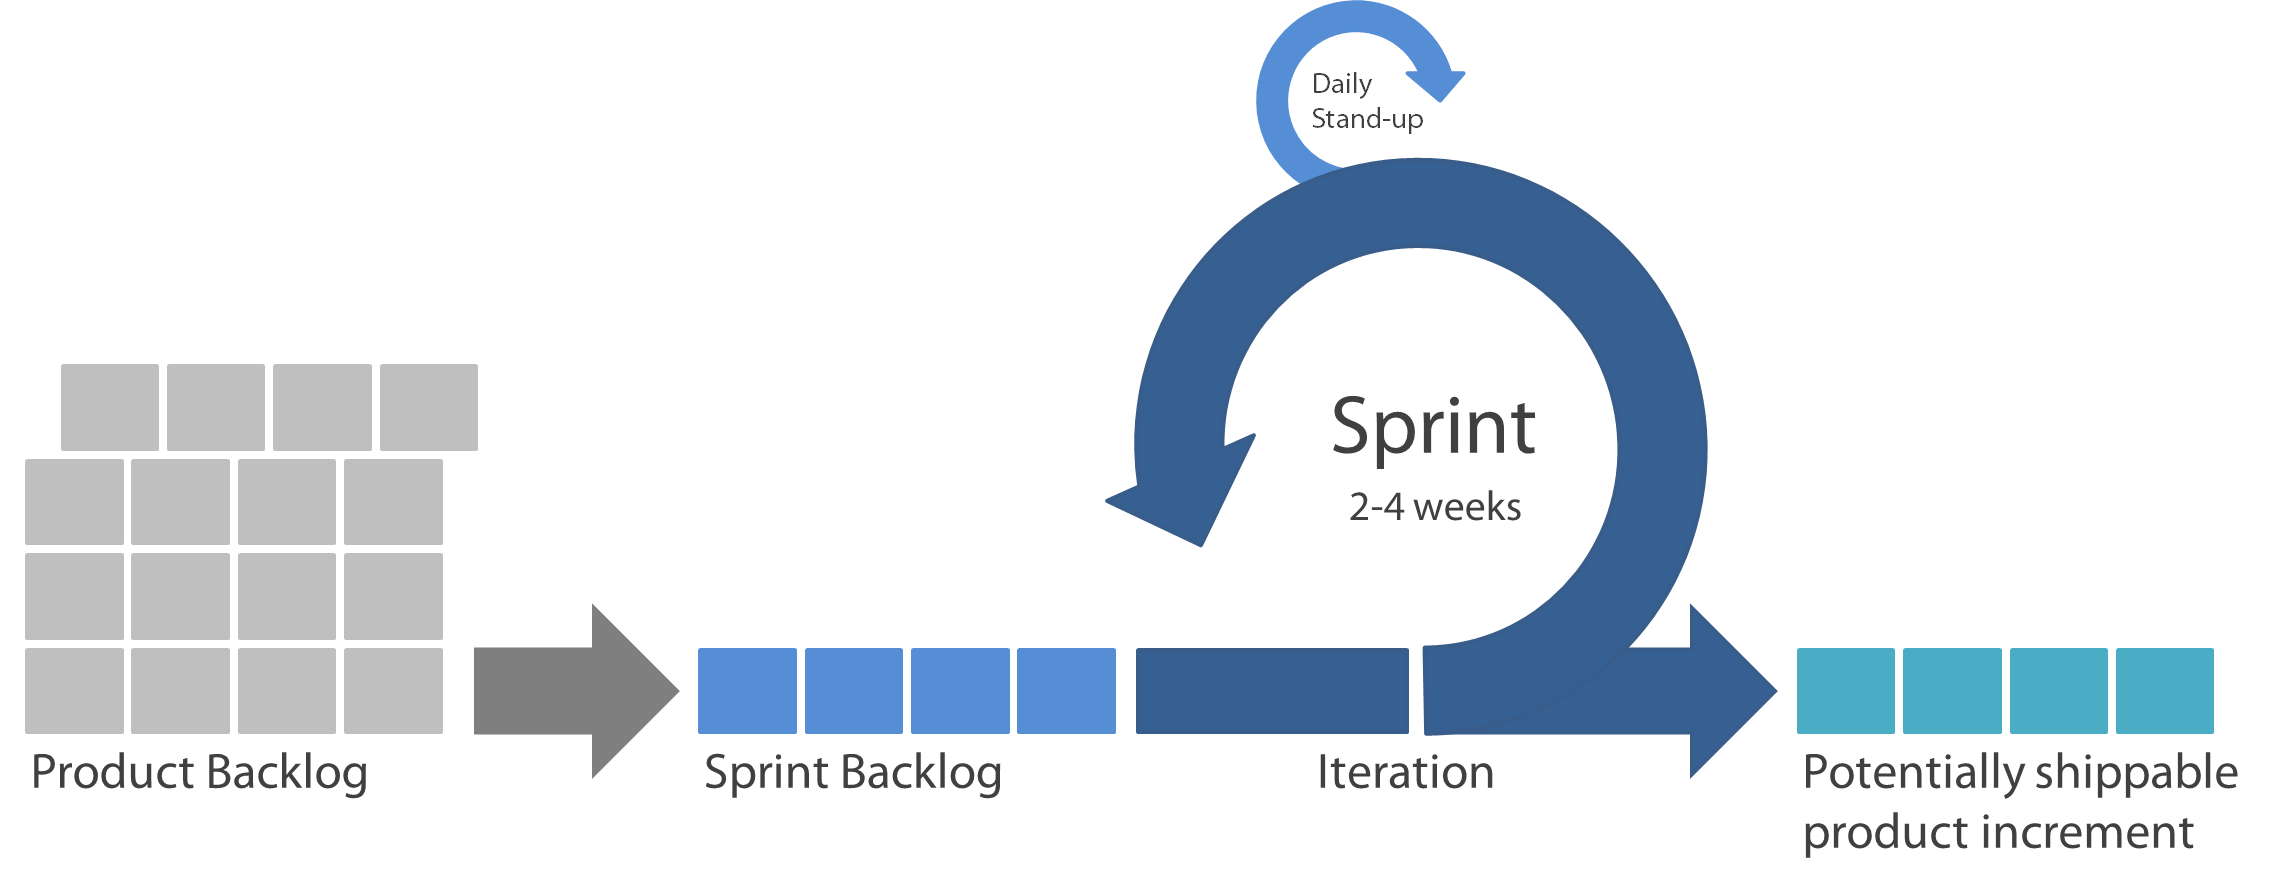
\includegraphics[width=12cm]{Pics/scrum.png}
\caption{Metodo agile scrum.}
\end{center}
\end{figure}
All'interno dell'azienda il lavoro viene organizzato secondo il metodo agile scrum.  \\
Il modello agile scrum prevede la suddivisione di un progetto in blocchi detti \textit{Sprint} ognuno dei quali deve produrre un avanzamento del software. Prevede, inoltre la suddivisione dei compiti in \textit{task}, che possono essere visti come una attività abbastanza piccola da essere svolta da una sola persona nell'arco di 4/8 ore. È previsto un rapporto a stretto contatto con il cliente e la pianificazione di frequenti meeting con la funzione di punti di controllo, dove verificare lo stato di avanzamento del progetto rispetto a quanto atteso.
È stato scelto questo modello poiché l'azienda sviluppa in maggioranza prodotti innovativi, quindi con tecnologie in evoluzione, e soggetti a continue variazioni dei requisiti rendendo necessaria un meccanismo di controllo flessibile. Nello specifico del progetto in analisi, la continua variazione delle norme di legge in vigore provoca continui mutamenti nell'implementazione del software ed un rapporto a stretto contatto con il cliente diventa indispensabile al fine di garantire la conformità del servizio.

\subsection{Strumenti a supporto dell'organizzazione del lavoro}
\subsubsection{Atlassian Suite}
\begin{figure}[H]
\begin{center}

\includegraphics[height=1.1cm]{Pics/atlassian_logo.png}
\caption{Logo della suite Atlassian}
\end{center}
\end{figure}
Per l'organizzazione del lavoro, ci si è appoggiati alla suite offerta da Atlassian, che fornisce tutti gli strumenti necessari alla gestione di codice e compiti. \\
Fa seguito l'elenco degli strumenti utilizzati a supporto delle principali necessità.

\subsubsection{Jira - Gestione dei Task e Sprint }
\begin{figure}[H]
\begin{center}

\includegraphics[height=1.4cm]{Pics/jira_logo.png}
\caption{Logo di Jira}
\end{center}
\end{figure}

Per la gestione dei \textit{Task} e degli \textit{Sprint} è stato utilizzato il software Jira della suite Atlassian.\\
Esso permette di creare ed assegnare i task alle persone le quali possono annotare il numero di ore dedicate ad ogni specifico task. È possibile inoltre avere una visione d'insieme dello sprint corrente e dei precedenti, pianificando anche i successivi.
È anche possibile collegare i task presenti su Jira con i \textit{commit} presenti su Bitbucket facendo riferimento nel testo del \textit{commit} al codice identificativo del \textit{task} tenendo sotto controllo l'evoluzione del codice per ogni \textit{task}.


\subsubsection{Confluence - Gestione  della documentazione}

\begin{figure}[H]
\begin{center}

\includegraphics[height=0.7cm]{Pics/confluence_logo.jpeg}
\caption{Logo di Confluence}
\end{center}
\end{figure}

Per la gestione della documentazione su norme aziendali e prodotti realizzati, viene utilizzato il software Confluence. Esso fornisce usa sorta di wiki integrato con tutte le applicazioni della suite collegata al progetto. Qui viene stesa la documentazione inerente a tutte le fasi del ciclo di vita del prodotto.

\subsubsection{Bitbucket - Versionamento}
\begin{figure}[H]
\begin{center}

\includegraphics[height=1cm]{Pics/bitbucket_logo.png}
\caption{Logo di Bitbucket}
\end{center}
\end{figure}

Per quanto riguarda il versionamento, viene utilizzato il servizio Bitbucket della suite. Esso utilizza \texttt{git} per la gestione del repository. 
 Per agevolare la cooperazione è stato adottato l'approccio \textbf{git-flow}. 

\subsubsection{Slack - Comunicazione}

\begin{figure}[htbp]
\begin{center}

\includegraphics[height=1cm]{Pics/slack_logo.png}
\caption{Logo di Slack}
\end{center}
\end{figure}

Per quanto riguarda la comunicazione interna ai membri dell'azienda è stato scelto di utilizzare il software gratuito Slack. 
Si tratta di un sistema di messaggistica che distingue le comunicazioni dirette a persone da quelle dirette a canali inerenti ad un particolare argomento. Le norme aziendali prevedono la creazione di un canale per ogni progetto.
Slack mette a disposizione anche un meccanismo di condivisione di file e, caratteristica essenziale, mantiene uno storico di tutti i messaggi di tutte le conversazioni al fine di mantenere un tracciamento delle comunicazioni interne. 
È fornita dal software anche una efficiente funzionalità di ricerca per recuperare le comunicazioni o i contenuti condivisi.
\subsubsection{Errbit - Rilevazione degli errori }

\begin{figure}[htbp]
\begin{center}

\includegraphics[height=1.4cm]{Pics/errbit_logo.png}
\caption{Logo di Errbit}
\end{center}
\end{figure}

Errbit è uno strumento per la rilevazione e gestione degli errori. Esso ha bisogno di un server dove girare e mantiene dei listener in ascolto dei messaggi di errore provenienti dall'applicazione alla quale è collegato.
Per ogni errore rilevato, vengono resi disponibili su una pagina web le informazioni relative alla tipologia dell'errore, il backTrace, l'utente per il quale è avvenuto, ed i parametri sottomessi alla pagina in analisi.
Sono inoltre esposte da questo framework delle API per AirBrake e Jira, in modo da favorirne l'integrazione.
Nello stage è stato fatto uso di questo framework nel server in produzione per essere a conoscenza con esattezza delle criticità del prodotto realizzato in modo da essere reattivi nella risoluzione dei bug rilevati.

\subsubsection{Airbrake - Gestione e notifica degli errori}

\begin{figure}[htbp]
\begin{center}

\includegraphics[height=1.6cm]{Pics/airbrake_logo.png}
\caption{Logo di Airbrake}
\end{center}
\end{figure}

Airbrake fornisce un sistema di notifiche push centralizzato. La sua caratteristica principale è quella di centralizzare la gestione delle notifiche permettendo un'accurata gestione dei flussi di spedizione dei messaggi e degli ambienti monitorati (sviluppo, staging, produzione). \\ 
È stato collegato Airbrake ad Errbit mediante le apposite API. 
Ad ogni eccezione catturata da ErrBit, AirBrake permette di visualizzare in una dashboard tutte le informazioni relative all'eccezione ed al contesto in cui essa è stata sollevata.  È inoltre possibile collegare Airbrake ad altri strumenti ad esempio per la gestione di report periodici. \\ 
 In questo progetto Airbrake è stato configurato in modo tale che le notifiche provenienti dal monitoraggio dell'ambiente di produzione siano spedite ad un canale di Slack appositamente creato.

%\st{
%Esso raccoglie tutti i messaggi provenienti dai sistemi cui è cui è associato (ad Esempio Errbit) e li inoltra nei flussi indicati nel pannello di configurazione mediante notifiche push. Nel caso di specie, sono sono stati associati i messaggi di errore provenienti dal server di produzione di ogni progetto, ad un canale di slack ad esso relativo.
%Ogni messaggio contiene le informazioni generali dell'errore oltre ad un collegamento ad una dashboard la quale, grazie al collegamento con Errbit, permette di analizzare i dettagli dell'errore e del contesto in cui è avvenuto.
%}

\cleardoublepage
\section{Il progetto di Stage}
Il progetto di stage consiste nell'estensione di un software web based, già sviluppato in azienda, a supporto delle aziende che intendono avvalersi dell’asseverazione in ambito della sicurezza sul lavoro, in particolare nel settore edilizio. \\
Con asseverazione si intende una scelta volontaria di una impresa edile al fine di dimostrare l'impegno per la prevenzione, salute e sicurezza nei luoghi di lavoro. Opera mediante la certificazione di conformità dei modelli di organizzazione e gestione aziendali e mediante visite a campione nei cantieri. L'asseverazione offre benefici economici alle aziende che la richiedono e garantisce efficacia esimente rispetto alla responsabilità amministrativa delle imprese.\\
Il software si pone come obiettivo la possibilità di fornire in ogni momento una fotografia dello stato della sicurezza in azienda, al fine di agevolarne il mantenimento nel tempo.\\
All'inserimento di nuove informazioni, verranno generate nuove domande, scadenze o vincoli. Se i risultati non sono conformi alle norme vigenti, verranno generati degli allarmi, che scompariranno solo nel momento in cui la violazione del vincolo che rappresentano non sia più verificata. \\
Dal punto di vista tecnico viene utilizzato un sistema esperto per mappare le norme in tema di sicurezza, individuare i punti deboli dell’azienda, ricordare al responsabile le scadenze, conservare ed indicizzare il patrimonio documentale in ambito sicurezza.
Il sistema ha una funzione proattiva e dinamica, variando gli allarmi in base alla variazione delle norme e allo stato dell’azienda (es. al crescere o diminuire del numero dei dipendenti, al variare della superficie delle sedi aziendali, dei cantieri...). La webapp si comporta quindi come un consulente digitale per l’azienda, aiutandola a mantenere aggiornato il suo modello di sicurezza e a rispettarlo.
Questo le permette all’azienda asseverata di accedere a significativi premi INAIL, di ottenere punti in graduatoria in bandi pubblici e di sollevare il datore di lavoro da responsabilità penali in caso di infortuni legati ad una mala gestione della sicurezza.

\subsection{Il prodotto esistente}

Il progetto è in una fase di sviluppo avanzato (versione alpha).
Alla data di inizio dello stage, il software supporta le aziende con i codici \gls{ATECO}\G\ in ambito edilizio, permette l’inserimento di informazioni su sedi, cantieri, dipendenti, organigramma aziendale e la gestione di abitabilità, certificato prevenzione incendi e della documentazione che emerge dal \gls{DVR}\G.
Vengono poste all'utente più di 400 domande per individuare lo stato di sicurezza. \\ 
Il sistema esperto è funzionante, ma va irrobustito e vanno implementate le regole opportune per individuare le criticità nei dati inseriti dall'utente.


\subsection{Obiettivi dello stage}

Il team ha l’obiettivo di rilasciare una versione beta del software entro la fine del 2015 e quindi procedere al primo test con l’utente finale, una importante azienda del settore edilizio, già  individuata.
Durante lo stage sono stati posti i seguenti obiettivi:
\begin{itemize}
\item Analisi di alcune logiche del sistema esperto in coordinamento con il cliente ed il consulente della sicurezza;
\item Progettazione delle funzionalità individuate nella fase di analisi;
\item Implementazione del risultato del punto precedente;
\item Stesura della documentazione relativa al codice prodotto;
\item Rendere il sistema più efficace, semplice ed usabile da parte di un utente competente in materia di sicurezza.
\end{itemize}

	\cleardoublepage
		% indice
	\pagestyle{roman}
	\setcounter{page}{3}
	\tableofcontents
	\clearpage
	\listoffigures
	\listoftables
	\cleardoublepage
	\abstract

	Il presente documento descrive il lavoro svolto durante il periodo di stage, della durata di circa trecento ore, dal laureando Fabio Ros presso l’azienda Moku S.r.l. 
	Il progetto di stage prevede l'analisi, la progettazione e lo sviluppo di alcune delle logiche del sistema esperto in coordinamento con il committente ed un consulente della sicurezza.
	Nello specifico è prevista l'implementazione delle componenti software sia lato backend, mediante l'utilizzo di Ruby on Rails, sia lato frontend simultaneamente alla definizione delle regole di gestione del sistema esperto utilizzando il framework Drools.

	\cleardoublepage
	%\vspace*{100pt}
\noindent \textbf{\LARGE Ringraziamenti}\\

\noindent \textit{Innanzitutto vorrei esprimere la mia gratitudine alla Prof.ssa Ombretta Gaggi, relatrice della mia tesi, per l'aiuto fornitomi e per la sua disponibilità durante la stesura del lavoro.\\
Desidero ringraziare con affetto i miei cari per il sostegno, il grande aiuto e per essermi stati vicini in ogni momento durante gli anni di studio.\\
Tengo molto a ringraziare i miei amici per i bei momenti passati assieme.}\\
\mbox{}\\
\noindent \textit{Padova, Aprile 2016} \\
\begin{flushright}
	Fabio Ros
\end{flushright}
	\cleardoublepage

	\pagestyle{plain}
	\section{Introduzione} 
\subsection{L'azienda}
\begin{figure}[H]
\begin{center}

\includegraphics[height=1.6cm]{Pics/logo_moku.jpg}
\caption{Logo dell'azienda ospitante - Moku S.r.l.}
\end{center}
\end{figure}
Moku S.r.l è una startup nata nel 2013 e situata in H-Farm. 
L'organizzazione del lavoro è supportata dalla suite Atlassian che offre un servizio cloud per la gestione dei compiti e dei progetti.
L'azienda lavora a stretto contatto con il cliente definendo requisiti, user experience dei prodotti realizzati ed opportunità di business.
Obiettivo primario dell'azienda è la qualità del software e l'utilizzo di tecnologie recenti poiché l'alto coefficiente innovativo dei prodotti realizzati rende necessaria una costante manutenzione che si vuole sia il più agevole possibile.

\subsubsection{Origine}
Il nome della startup, in hawaiiano, significa \textit{isola}. Questo perché l'idea iniziale era una applicazione web per studenti dove un \textit{"moku"} era visto come uno spazio personale (un’isola), ma allo stesso tempo uno spazio di collaborazione, rappresentando un \textit{arcipelago} di isole collegate tra loro.
In origine si basava sulla realizzazione di una applicazione il cui uso era riservato principalmente agli studenti. Ad ogni utente era data la possibilità di caricare i propri documenti in diverse tipologie di formato. Una volta aperti, era possibile prendere degli appunti su un layer posto sopra al documento caricato. Questo può essere condiviso con i propri collaboratori. Era anche possibile registrare la lezione e mettere delle note anche alla traccia audio, la quale si poteva sincronizzare con un particolare documento.
\subsubsection{Evoluzione}
Ora le attività dell'azienda si concentrano nella consulenza IT, in particolare nella realizzazione di software innovativo a supporto delle esigenze concrete dei clienti. Il progetto da me svolto è un chiaro esempio di questo mutamento, infatti il prodotto finito risulterà di completa proprietà di un'azienda esterna.  \\ Ora l'azienda, quindi, sviluppa solo marginalmente software proprietario, ma sviluppa principalmente su commissione di aziende esterne.

\subsection{Organizzazione del lavoro}
\begin{figure}[H]
\begin{center}
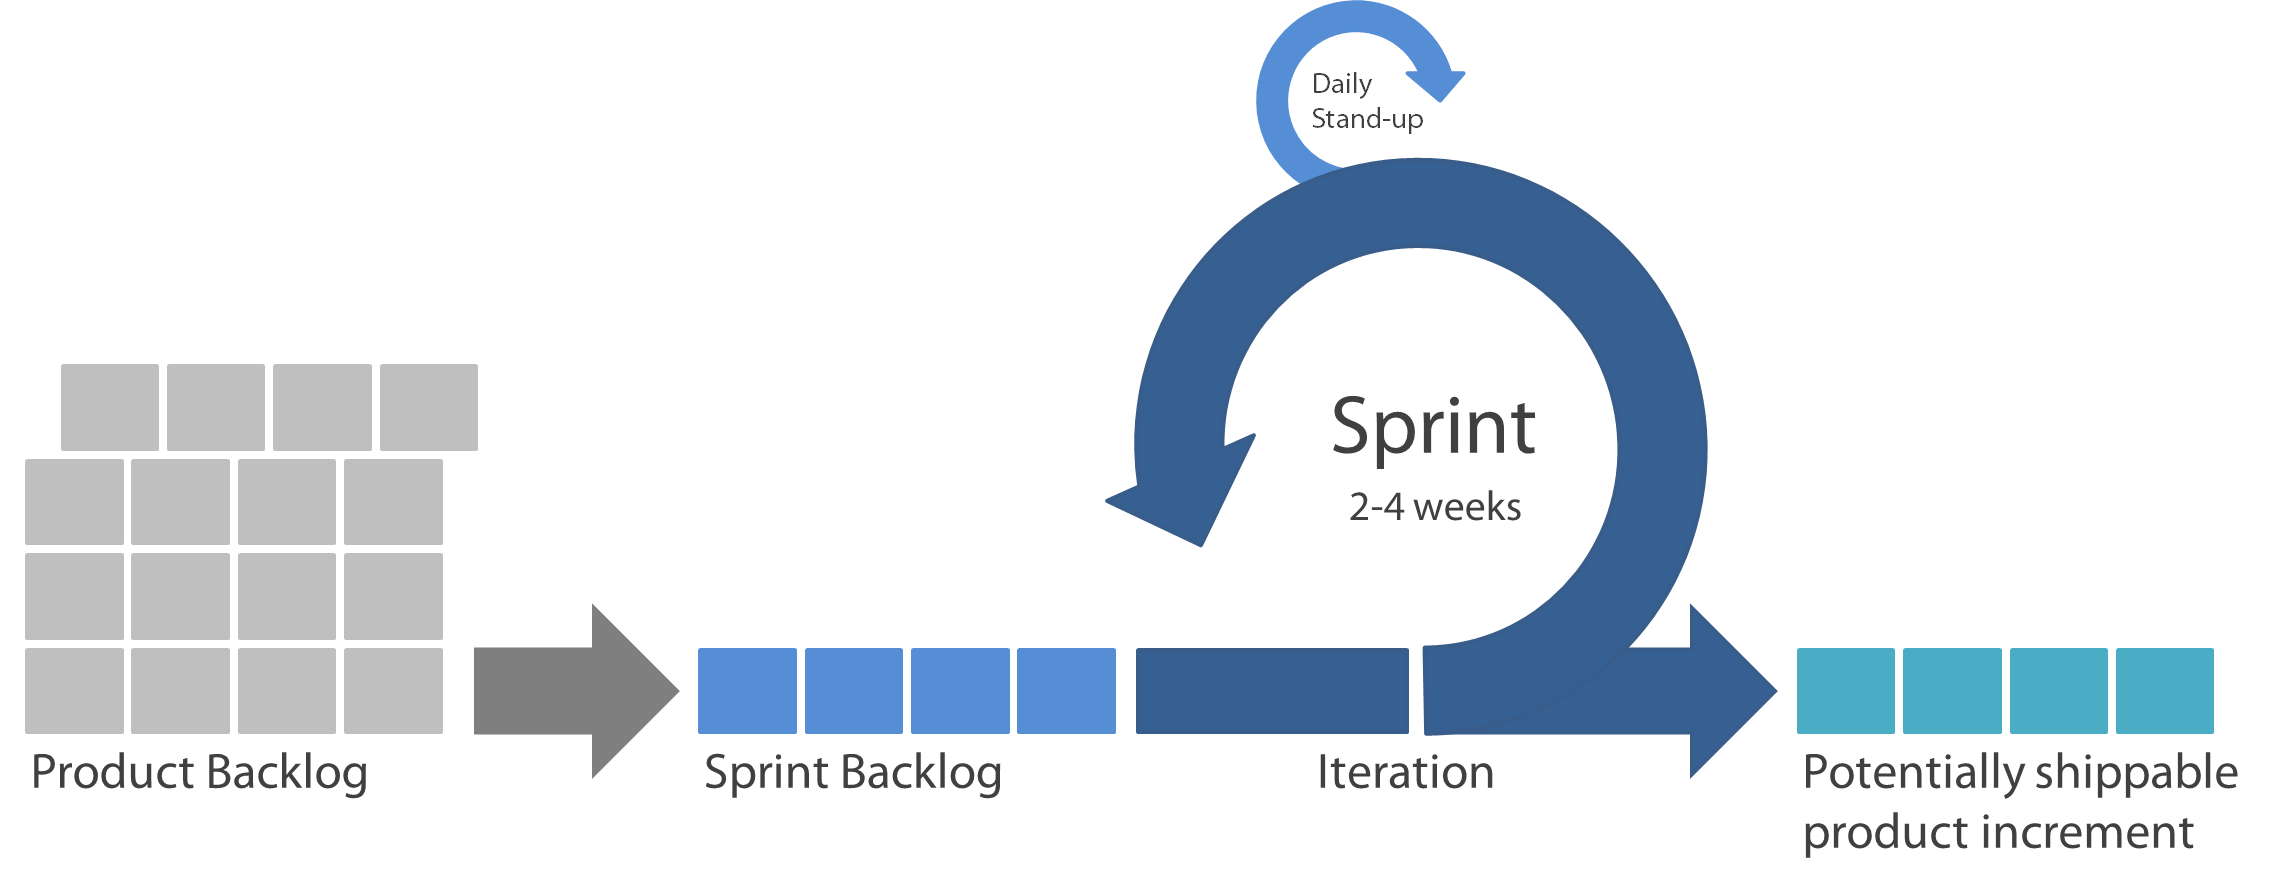
\includegraphics[width=12cm]{Pics/scrum.png}
\caption{Metodo agile scrum.}
\end{center}
\end{figure}
All'interno dell'azienda il lavoro viene organizzato secondo il metodo agile scrum.  \\
Il modello agile scrum prevede la suddivisione di un progetto in blocchi detti \textit{Sprint} ognuno dei quali deve produrre un avanzamento del software. Prevede, inoltre la suddivisione dei compiti in \textit{task}, che possono essere visti come una attività abbastanza piccola da essere svolta da una sola persona nell'arco di 4/8 ore. È previsto un rapporto a stretto contatto con il cliente e la pianificazione di frequenti meeting con la funzione di punti di controllo, dove verificare lo stato di avanzamento del progetto rispetto a quanto atteso.
È stato scelto questo modello poiché l'azienda sviluppa in maggioranza prodotti innovativi, quindi con tecnologie in evoluzione, e soggetti a continue variazioni dei requisiti rendendo necessaria un meccanismo di controllo flessibile. Nello specifico del progetto in analisi, la continua variazione delle norme di legge in vigore provoca continui mutamenti nell'implementazione del software ed un rapporto a stretto contatto con il cliente diventa indispensabile al fine di garantire la conformità del servizio.

\subsection{Strumenti a supporto dell'organizzazione del lavoro}
\subsubsection{Atlassian Suite}
\begin{figure}[H]
\begin{center}

\includegraphics[height=1.1cm]{Pics/atlassian_logo.png}
\caption{Logo della suite Atlassian}
\end{center}
\end{figure}
Per l'organizzazione del lavoro, ci si è appoggiati alla suite offerta da Atlassian, che fornisce tutti gli strumenti necessari alla gestione di codice e compiti. \\
Fa seguito l'elenco degli strumenti utilizzati a supporto delle principali necessità.

\subsubsection{Jira - Gestione dei Task e Sprint }
\begin{figure}[H]
\begin{center}

\includegraphics[height=1.4cm]{Pics/jira_logo.png}
\caption{Logo di Jira}
\end{center}
\end{figure}

Per la gestione dei \textit{Task} e degli \textit{Sprint} è stato utilizzato il software Jira della suite Atlassian.\\
Esso permette di creare ed assegnare i task alle persone le quali possono annotare il numero di ore dedicate ad ogni specifico task. È possibile inoltre avere una visione d'insieme dello sprint corrente e dei precedenti, pianificando anche i successivi.
È anche possibile collegare i task presenti su Jira con i \textit{commit} presenti su Bitbucket facendo riferimento nel testo del \textit{commit} al codice identificativo del \textit{task} tenendo sotto controllo l'evoluzione del codice per ogni \textit{task}.


\subsubsection{Confluence - Gestione  della documentazione}

\begin{figure}[H]
\begin{center}

\includegraphics[height=0.7cm]{Pics/confluence_logo.jpeg}
\caption{Logo di Confluence}
\end{center}
\end{figure}

Per la gestione della documentazione su norme aziendali e prodotti realizzati, viene utilizzato il software Confluence. Esso fornisce usa sorta di wiki integrato con tutte le applicazioni della suite collegata al progetto. Qui viene stesa la documentazione inerente a tutte le fasi del ciclo di vita del prodotto.

\subsubsection{Bitbucket - Versionamento}
\begin{figure}[H]
\begin{center}

\includegraphics[height=1cm]{Pics/bitbucket_logo.png}
\caption{Logo di Bitbucket}
\end{center}
\end{figure}

Per quanto riguarda il versionamento, viene utilizzato il servizio Bitbucket della suite. Esso utilizza \texttt{git} per la gestione del repository. 
 Per agevolare la cooperazione è stato adottato l'approccio \textbf{git-flow}. 

\subsubsection{Slack - Comunicazione}

\begin{figure}[htbp]
\begin{center}

\includegraphics[height=1cm]{Pics/slack_logo.png}
\caption{Logo di Slack}
\end{center}
\end{figure}

Per quanto riguarda la comunicazione interna ai membri dell'azienda è stato scelto di utilizzare il software gratuito Slack. 
Si tratta di un sistema di messaggistica che distingue le comunicazioni dirette a persone da quelle dirette a canali inerenti ad un particolare argomento. Le norme aziendali prevedono la creazione di un canale per ogni progetto.
Slack mette a disposizione anche un meccanismo di condivisione di file e, caratteristica essenziale, mantiene uno storico di tutti i messaggi di tutte le conversazioni al fine di mantenere un tracciamento delle comunicazioni interne. 
È fornita dal software anche una efficiente funzionalità di ricerca per recuperare le comunicazioni o i contenuti condivisi.
\subsubsection{Errbit - Rilevazione degli errori }

\begin{figure}[htbp]
\begin{center}

\includegraphics[height=1.4cm]{Pics/errbit_logo.png}
\caption{Logo di Errbit}
\end{center}
\end{figure}

Errbit è uno strumento per la rilevazione e gestione degli errori. Esso ha bisogno di un server dove girare e mantiene dei listener in ascolto dei messaggi di errore provenienti dall'applicazione alla quale è collegato.
Per ogni errore rilevato, vengono resi disponibili su una pagina web le informazioni relative alla tipologia dell'errore, il backTrace, l'utente per il quale è avvenuto, ed i parametri sottomessi alla pagina in analisi.
Sono inoltre esposte da questo framework delle API per AirBrake e Jira, in modo da favorirne l'integrazione.
Nello stage è stato fatto uso di questo framework nel server in produzione per essere a conoscenza con esattezza delle criticità del prodotto realizzato in modo da essere reattivi nella risoluzione dei bug rilevati.

\subsubsection{Airbrake - Gestione e notifica degli errori}

\begin{figure}[htbp]
\begin{center}

\includegraphics[height=1.6cm]{Pics/airbrake_logo.png}
\caption{Logo di Airbrake}
\end{center}
\end{figure}

Airbrake fornisce un sistema di notifiche push centralizzato. La sua caratteristica principale è quella di centralizzare la gestione delle notifiche permettendo un'accurata gestione dei flussi di spedizione dei messaggi e degli ambienti monitorati (sviluppo, staging, produzione). \\ 
È stato collegato Airbrake ad Errbit mediante le apposite API. 
Ad ogni eccezione catturata da ErrBit, AirBrake permette di visualizzare in una dashboard tutte le informazioni relative all'eccezione ed al contesto in cui essa è stata sollevata.  È inoltre possibile collegare Airbrake ad altri strumenti ad esempio per la gestione di report periodici. \\ 
 In questo progetto Airbrake è stato configurato in modo tale che le notifiche provenienti dal monitoraggio dell'ambiente di produzione siano spedite ad un canale di Slack appositamente creato.

%\st{
%Esso raccoglie tutti i messaggi provenienti dai sistemi cui è cui è associato (ad Esempio Errbit) e li inoltra nei flussi indicati nel pannello di configurazione mediante notifiche push. Nel caso di specie, sono sono stati associati i messaggi di errore provenienti dal server di produzione di ogni progetto, ad un canale di slack ad esso relativo.
%Ogni messaggio contiene le informazioni generali dell'errore oltre ad un collegamento ad una dashboard la quale, grazie al collegamento con Errbit, permette di analizzare i dettagli dell'errore e del contesto in cui è avvenuto.
%}

\cleardoublepage
\section{Il progetto di Stage}
Il progetto di stage consiste nell'estensione di un software web based, già sviluppato in azienda, a supporto delle aziende che intendono avvalersi dell’asseverazione in ambito della sicurezza sul lavoro, in particolare nel settore edilizio. \\
Con asseverazione si intende una scelta volontaria di una impresa edile al fine di dimostrare l'impegno per la prevenzione, salute e sicurezza nei luoghi di lavoro. Opera mediante la certificazione di conformità dei modelli di organizzazione e gestione aziendali e mediante visite a campione nei cantieri. L'asseverazione offre benefici economici alle aziende che la richiedono e garantisce efficacia esimente rispetto alla responsabilità amministrativa delle imprese.\\
Il software si pone come obiettivo la possibilità di fornire in ogni momento una fotografia dello stato della sicurezza in azienda, al fine di agevolarne il mantenimento nel tempo.\\
All'inserimento di nuove informazioni, verranno generate nuove domande, scadenze o vincoli. Se i risultati non sono conformi alle norme vigenti, verranno generati degli allarmi, che scompariranno solo nel momento in cui la violazione del vincolo che rappresentano non sia più verificata. \\
Dal punto di vista tecnico viene utilizzato un sistema esperto per mappare le norme in tema di sicurezza, individuare i punti deboli dell’azienda, ricordare al responsabile le scadenze, conservare ed indicizzare il patrimonio documentale in ambito sicurezza.
Il sistema ha una funzione proattiva e dinamica, variando gli allarmi in base alla variazione delle norme e allo stato dell’azienda (es. al crescere o diminuire del numero dei dipendenti, al variare della superficie delle sedi aziendali, dei cantieri...). La webapp si comporta quindi come un consulente digitale per l’azienda, aiutandola a mantenere aggiornato il suo modello di sicurezza e a rispettarlo.
Questo le permette all’azienda asseverata di accedere a significativi premi INAIL, di ottenere punti in graduatoria in bandi pubblici e di sollevare il datore di lavoro da responsabilità penali in caso di infortuni legati ad una mala gestione della sicurezza.

\subsection{Il prodotto esistente}

Il progetto è in una fase di sviluppo avanzato (versione alpha).
Alla data di inizio dello stage, il software supporta le aziende con i codici \gls{ATECO}\G\ in ambito edilizio, permette l’inserimento di informazioni su sedi, cantieri, dipendenti, organigramma aziendale e la gestione di abitabilità, certificato prevenzione incendi e della documentazione che emerge dal \gls{DVR}\G.
Vengono poste all'utente più di 400 domande per individuare lo stato di sicurezza. \\ 
Il sistema esperto è funzionante, ma va irrobustito e vanno implementate le regole opportune per individuare le criticità nei dati inseriti dall'utente.


\subsection{Obiettivi dello stage}

Il team ha l’obiettivo di rilasciare una versione beta del software entro la fine del 2015 e quindi procedere al primo test con l’utente finale, una importante azienda del settore edilizio, già  individuata.
Durante lo stage sono stati posti i seguenti obiettivi:
\begin{itemize}
\item Analisi di alcune logiche del sistema esperto in coordinamento con il cliente ed il consulente della sicurezza;
\item Progettazione delle funzionalità individuate nella fase di analisi;
\item Implementazione del risultato del punto precedente;
\item Stesura della documentazione relativa al codice prodotto;
\item Rendere il sistema più efficace, semplice ed usabile da parte di un utente competente in materia di sicurezza.
\end{itemize}

	\cleardoublepage
	\subsection{Pianificazione del lavoro}

%stima iniziale
La pianificazione iniziale del lavoro prevedeva la distribuzione delle trecento ore nel modo seguente:
\begin{enumerate}
	\item	40 ore:     studio di Ruby on Rails, Drools e del software esistente;
	\item	50 ore:		analisi dei requisiti e dei miglioramenti da effettuare al codice esistente
	\item	40ore:		riprogettazione delle componenti esistenti che presentano criticità e delle nuove componenti
	\item	100 ore:     codifica di funzionalità e test;
	\item	40 ore:		implementazione delle regole Drools;
	\item 	15 ore:		 stesura della documentazione;
	\item	15 ore: 	verifica.
\end{enumerate}

%
%\begin{figure}[H]
%	\begin{center}
%		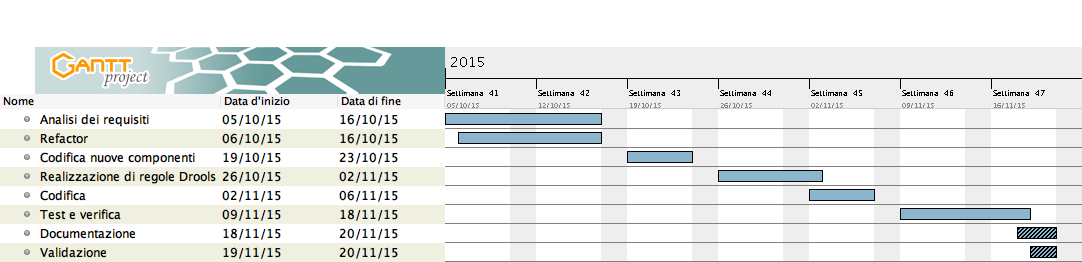
\includegraphics[width=16cm]{Pics/gantt.png}
%		\caption{Diagramma di Gantt.}
%		\label{fig:Gantt}
%	\end{center}
%\end{figure}
%


Durante lo stage, le ore sono state mantenute tali e quali alle previsioni. Tuttavia, la loro distribuzione nel tempo è leggermente cambiata rispetto al piano di lavoro. \\
L'attività di sviluppo è stata divisa in due parti distinte:  la prima relativa alla riprogettazione e codifica delle componenti già presenti al momento dell'inizio dello stage, la seconda relativa allo sviluppo delle nuove componenti.
A seguito di una riunione con il committente, si sono rese necessarie alcune modifiche che hanno provocato una leggera variazione del piano di lavoro.\\

Nello specifico l'ordine di esecuzione con le relative ore impiegate sono state le seguenti:
\begin{enumerate}
	\item	40 ore:     studio di Ruby on Rails, Drools e del software esistente;
	\item	20 ore:     rilevamento delle  criticità sulle componenti esistenti ;
	\item	30 ore:		analisi dei requisiti
	\item	15 ore:		riprogettazione delle componenti esistenti che presentano criticità
	\item	20 ore:     progettazione delle nuove entità richieste;
	\item	80 ore:     codifica di funzionalità e test;
	\item	4 ore:       colloquio con il committente per validare le nuove modifiche;
	\item 	4 ore:		 riprogettazione delle componenti da modificare;
	\item  	22 ore:	 	codifica di funzionalità e test;
	\item	40 ore:		implementazione delle regole Drools;
	\item 	15 ore:		 stesura della documentazione;
	\item	15 ore: 	verifica.
\end{enumerate}

Il conteggio totale delle ore al termine dello stage è di trecentocinque.
Data la complessità del progetto, le ore disponibili sono state sufficienti alla realizzazione delle funzionalità tali da soddisfare tutti i requisiti obbligatori e desiderabili, ma nessuno di quelli opzionali.
	\cleardoublepage
	\section{Analisi del prodotto esistente}

Al momento dell'arrivo in azienda era già presente una versione alpha del software. \\
Le aziende che il prodotto si prefigge di supportare in questa fase, sono quelle con i codici \gls{ATECO}\G\ in ambito edilizio. In particolare, al mio arrivo erano gestite le informazioni relative a:
\begin{itemize}
	\item Sedi;
	\item Cantieri;
	\item Dipendenti;
	\item Organigramma aziendale;
	\item Abitabilità;
	\item Certificato di prevenzione degli incendi;
	\item \gls{DVR}\G\ e documentazione collaterale ad esso.
\end{itemize}
Il software esponeva una collezione di oltre 400 domande. Sulla base delle risposte a queste domande ed alle informazioni relative alle entità sopra indicate, venivano verificati alcuni vincoli mediante regole del sistema esperto.

\subsection{Architettura del software}
\subsubsection{Architettura ad alto livello}
Il software è gestito mediante tecnologia \gls{SaaS}\G, un modello di distribuzione del software applicativo dove il fornitore del software si occupa della sua implementazione e manutenzione. Il servizio viene erogato al cliente mediante una applicazione web fruibile via internet. \\ 
L'applicazione web risiede fisicamente su una macchina virtuale della piattaforma cloud \gls{AWS}\G, al fine di evitare oneri e spese di gestione di una infrastruttura informatica dedicata e garantire la scalabilità del servizio.\\

Come è possibile osservare nella \autoref{fig:Architettura}, ogni istanza di macchina virtuale contiene un clone dell'intera architettura. È stata scelta questa soluzione perché è prevista la possibilità di vendere il pacchetto a più utenti che possono fungere da distributori.\\
Ogni istanza è composta da quattro componenti principali:
\begin{itemize}
	\item \textit{Rule Engine;}
	\item \textit{Database;}
	\item \textit{Web Application;}
	\item \textit{Storage.}
\end{itemize}
La componente \textit{Storage}, in particolare, è stata dedicata al salvataggio di documenti in formato PDF esportabili in ogni momento da ogni azienda. Questa funzionalità non è ancora stata implementata. \\
Il routing delle richieste viene effettuato con un \gls{reverse proxy}\G, nello specifico \textit{NGINX}. \\
In particolare Ruby on Rails permette nativamente di creare e versionare i database a seconda dell'ambiente nel quale si opera (\textit{development, test, staging e production}). Questa caratteristica è tornata molto utile per lo sviluppo, dal momento che è stato possibile fare test accurati senza intaccare i dati in produzione. Inoltre ciò rende possibile evitare di utilizzare la console in sandbox di Rails, la quale presenta criticità nella consistenza dei dati visibili da shell ripetto a quelli visibili da \gls{browser}\G. \\
La persistenza dei dati è stata gestita mediante il modulo \texttt{ActiveRecord} di Ruby on Rails (descritto nella sezione \ref{sec:ActiveRecord}) il quale salva le informazioni su un database \textit{ PostgreSQL}.
\begin{figure}[H]
	\begin{center}
		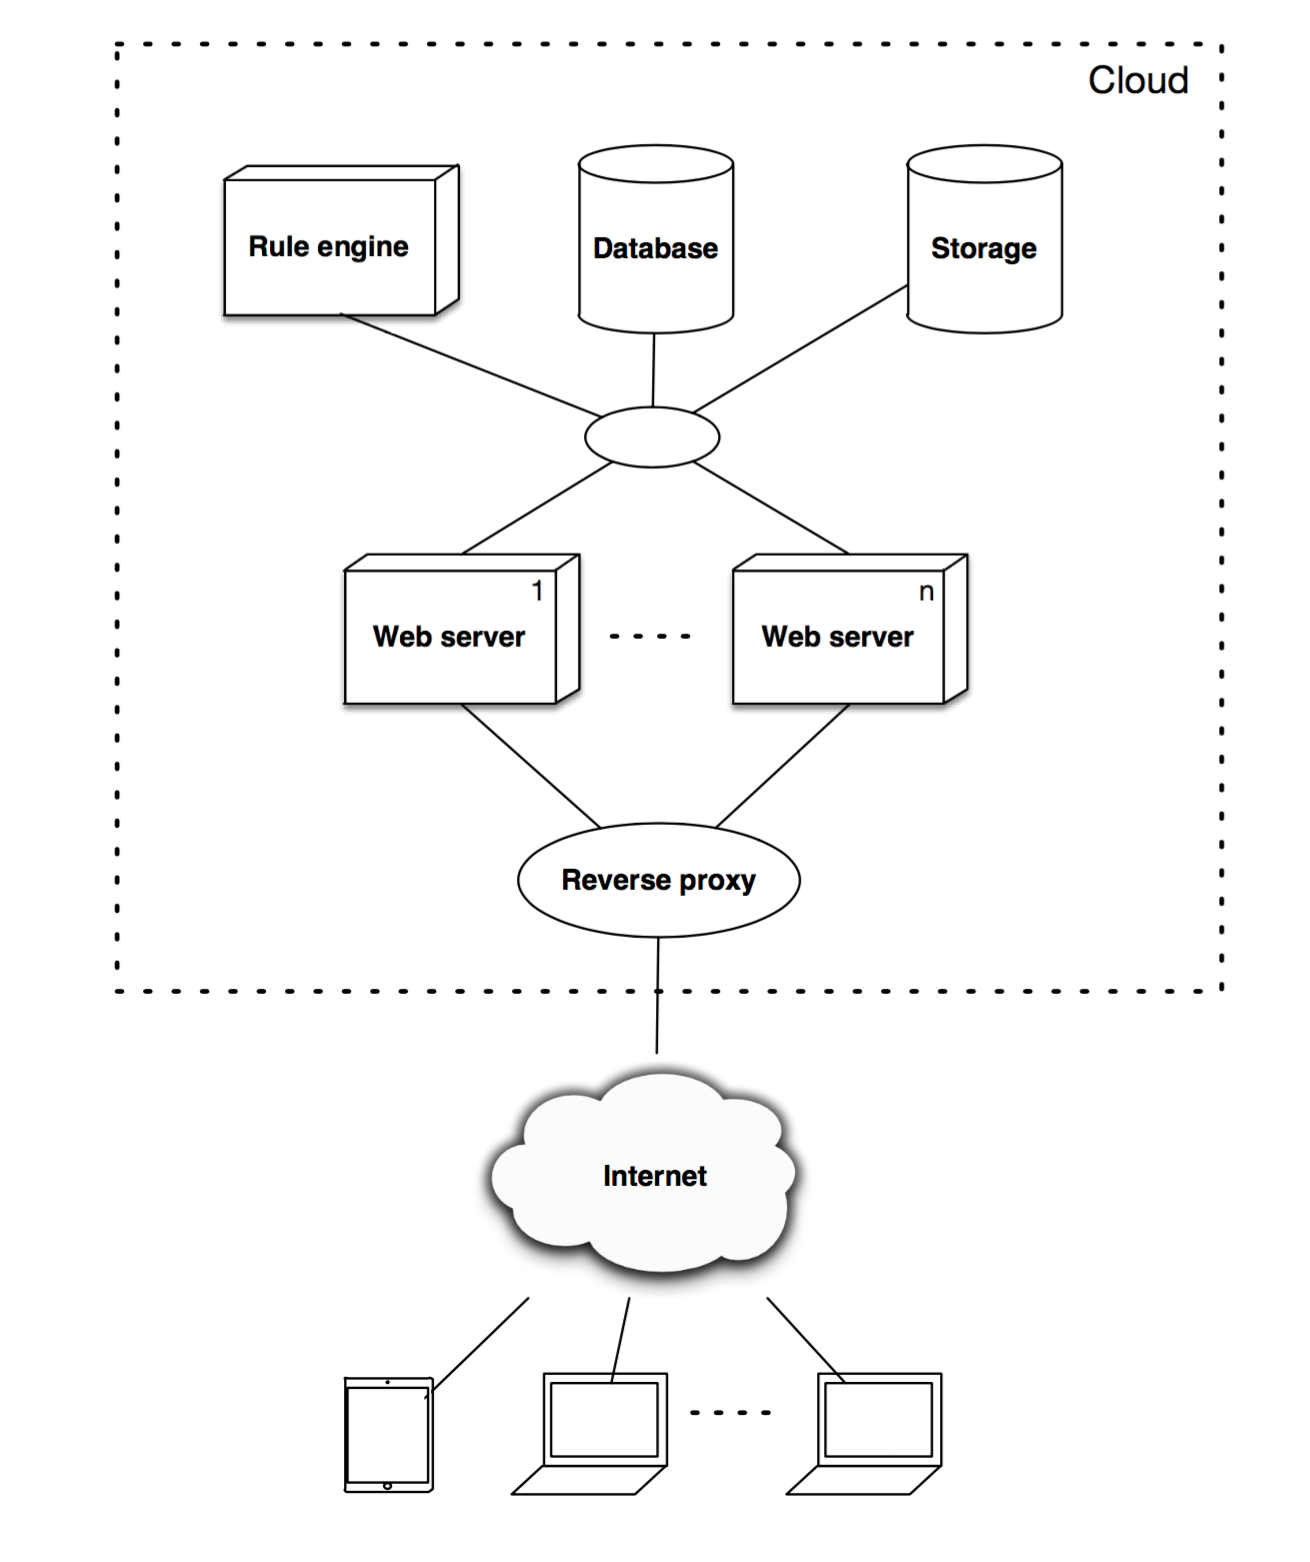
\includegraphics[width=16cm]{Pics/architettura.png}
		\caption{Architettura del sistema}
		\label{fig:Architettura}
	\end{center}
\end{figure}

\subsubsection{Architettura a basso livello}
L'applicazione web è organizzata secondo il pattern \gls{MVC}\G. Per il raggiungimento delle viste e l'accesso alle informazioni necessarie al corretto funzionamento dell'applicazione è stata implementata una interfaccia \gls{REST}\G. \\
Il sistema ha come entità principale il modello \texttt{Company} al quale sono riferite, direttamente o indirettamente, tutte le risorse.\\ 
Sono poi presenti numerosi modelli relativi alle entità che partecipano alla procedura di \gls{asseverazione}\G.
I modelli più significativi sono:
\begin{itemize} 
	\item \texttt{Alert} per rappresentare gli allarmi;
	\item \texttt{Answer} per rappresentare le risposte alle domande;
	\item \texttt{Company} per rappresentare una azienda;
	\item \texttt{ConstructionSite} per rappresentare un cantiere;
	\item \texttt{Dpi} per rappresentare un dispositivo di protezione individuale;
	\item \texttt{Duty} per rappresentare una mansione;
	\item \texttt{FireExtinguisher}  per rappresentare un estintore;
	\item \texttt{FirstAidBox} per rappresentare una cassetta di primo soccorso;
	\item \texttt{Individual} per rappresentare una persona;
	\item \texttt{Location} per rappresentare un edificio aziendale, ovvero una sede operativa, una sede amministrativa, una sede legale oppure un magazzino;
	\item \texttt{Machine, LiftingEquipment, ElectricTool}  per rappresentare un mezzo oppure uno strumento presente nel parco macchine;
	\item \texttt{MedicalVisit} per rappresentare una visita medica;
	\item \texttt{Procedure} per rappresentare una procedura aziendale, sia essa di prassi o di sistema;
	\item \texttt{Question} per rappresentare una domanda;
	\item \texttt{Training} per rappresentare un corso.
\end{itemize}	
Per ciascun modello, sono stati realizzati opportuni \textit{controller} e \textit{viste}. \\
Sono stati implementati, inoltre numerosi \gls{concern}\G\ per modularizzare le funzionalità indipendenti dalla singola classe ed allo stesso tempo riutilizzabili da altre classi. Ad esempio, ogni modello che, se istanziato, provoca un aumento del numero delle domande in attesa di risposta, include un apposito \gls{concern}\G\ per l'aggiornamento di un contatore dedicato a tale scopo. Per il calcolo del valore, il \gls{concern}\G\ ricava il nome della classe dell'oggetto corrente mediante \gls{reflection}\G\ ed incrementa automaticamente il valore del numero di domande correlate al tipo individuato.\\

\paragraph*{Relazioni tra domande, risposte ed allarmi}\mbox{} \\
\hl{Per facilitare la comprensione di alcune delle soluzioni descritte di seguito è importante essere a conoscenza delle relazioni presenti tra domande, risposte ed allarmi.}\\
Le risposte sono direttamente collegate alle domande ed ad una entità. \\Quando un utente risponde ad una domanda, viene aggiornato il recod relativo a quella risposta.\\
A seguito di un inserimento o aggiornamento di una risposta, interviene Drools che valuta se le informazioni inserite rispettano tutti i vincoli previsti, altrimenti viene sollevato un allarme. \\ 
Per questioni di efficienza, gli allarmi relativi al vincolo di presenza  di una risposta, vengono gestiti direttamente dalle funzionalità di validazione di Rails.\\
Come per le risposte, anche gli allarmi sono sempre collegati ad una risorsa, che di default è l'azienda corrente, ma può assumere come valore una qualsiasi istanza di un modello, purché non sia nulla.
Particolarmente degna di nota è l'associazione di una risposta o di un \textit{allarme} alla relativa risorsa. Per fare ciò si è utilizzato l'approccio standard di Rails per il supporto alle associazioni polimorfe. \\  
Come si può vedere da  \autoref{fig:DiagrammaClassiAssociazioniPolimorfe}, indicando il tipo e l'id della risorsa interessata, l'accesso avviene tramite valutazione della classe e ricerca del relativo \textit{id}. \\
Si può pensare, ad esempio, all'allarme scatenato alla scadenza di un estintore. \\
La Risposta (\textit{Answer}) avrà i due campi \texttt{answerable\_type} ed \texttt{answerable\_id} impostati rispettivamente a \textit{"FireExtinguisher"} ed al suo \textit{id}.  L'allarme avrà un riferimento alla domanda per la quale è stata data una risposta. In questo modo è possibile conoscere il punto esatto dove dirottare l'utente al click sull'allarme per raggiungere il punto di non conformità. Questo aspetto è stato considerato di fondamentale importanza poiché la mole delle informazioni nel software è molto grande, è quindi necessario fornire il maggior numero di strumenti possibili all'utente per facilitarne la navigazione e l'orientamento nel sistema.
\begin{figure}[H]
	\begin{center}
		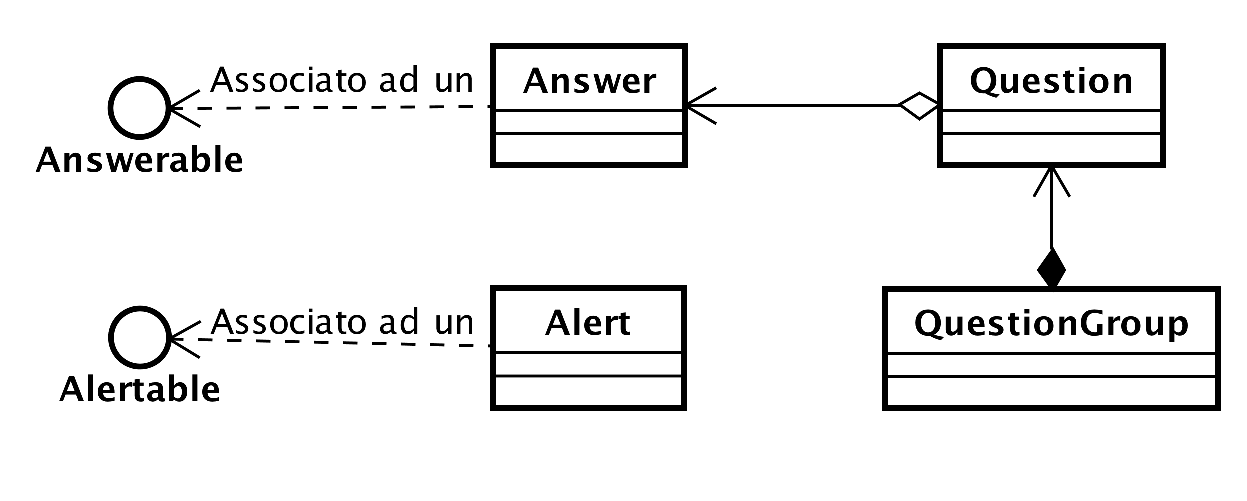
\includegraphics[width=14cm]{Pics/diagramma_classi_associazioni_polimorfe.png}
		\caption{Diagramma delle classi delle associazioni polimorfe di Risposte ed Allarmi.}
		\label{fig:DiagrammaClassiAssociazioniPolimorfe}
	\end{center}
\end{figure}

\subsubsection{Integrazione tra Ruby on Rails e Drools}\mbox{} \\

Il codice è stato scritto per la maggior parte utilizzando Ruby on Rails ma il rule engine (Drools) è un \gls{framework}\G\ scritto in Java. I due linguaggi non sono nativamente compatibili. \\
Per ovviare a questo problema, è stato utilizzato JRuby, un interprete del linguaggio Ruby scritto in Java, quindi in esecuzione su una \gls{JVM}\G. \\
Per il corretto funzionamento di Drools, è necessario inserire le informazioni nella \textit{Working Memory} come \textit{"fatti"} che sono richiesti come oggetti di tipo \gls{JavaBean}\G\ o \gls{POJO}\G.\\
Per far cooperare i due ambienti, è stato implementato un apposito \gls{concern}\G\ chiamato \texttt{"act\_as\_fact"}. Questo modulo viene incluso nelle classi delle quali è necessario tenere traccia nella \textit{Working Memory} e vengono generati, mediante \gls{reflection} utilizzando i template di Rails (\gls{ERB}\G), le classi Java corrispondenti.


\newpage
\subsubsection{Flusso dei dati ed interazione}

 Un aspetto che merita di essere esaminato è il flusso con il quale vengono generate e valutate domande e risposte .
\begin{figure}[H]
	\begin{center}
		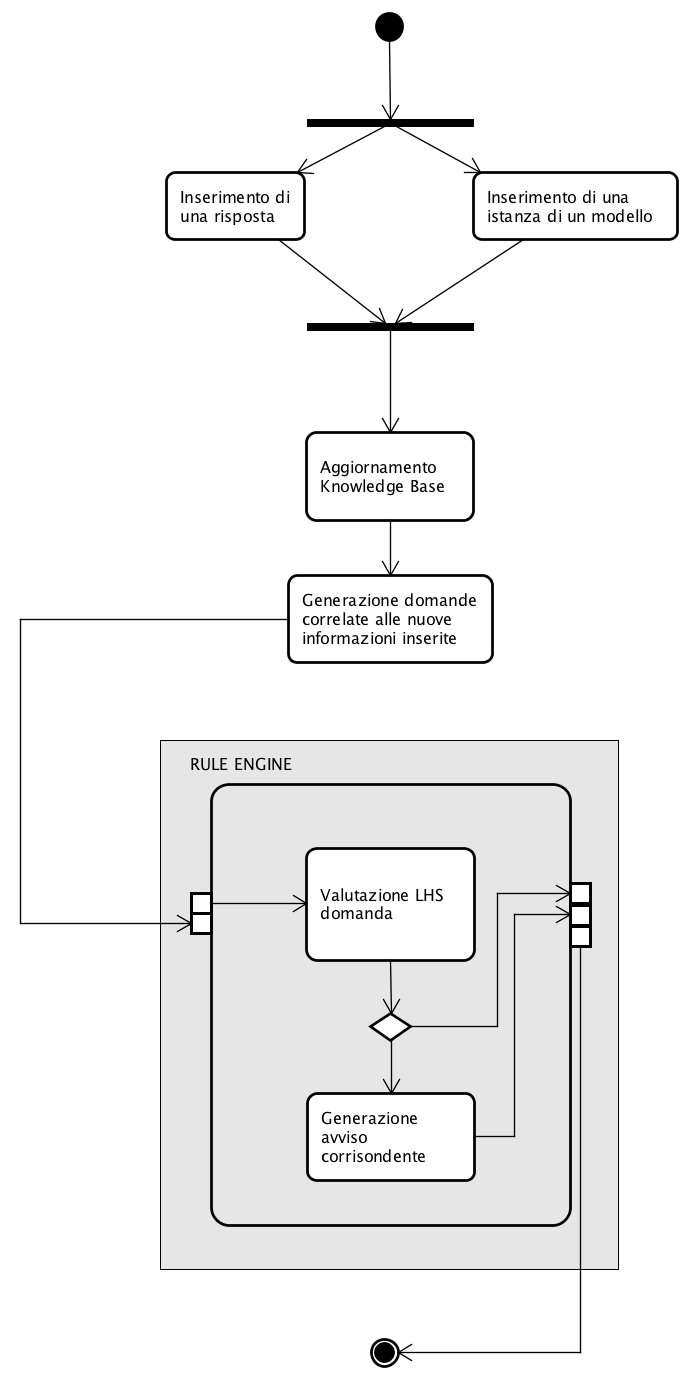
\includegraphics[width=8cm]{Pics/diagramma_attivita_risposte.png}
		\caption{Diagramma di attività del flusso di una risposta o l'inserimento di un oggetto a modello}
		\label{fig:DiagrammaAttivitaRisposte}
	\end{center}
\end{figure}

Come è possibile osservare dalla \autoref{fig:DiagrammaAttivitaRisposte}, nel momento in cui un utente inserisce o modifica un'istanza di un modello oppure risponde ad una domanda, viene aggiornata la \textit{Working Memory}. \\
Nel caso un cui venga generata o aggiornata un'istanza di modello, può essere necessario l'inserimento di alcune domande ad essa direttamente correlate.\\
Un esempio è rappresentato dall'aggiunta di un estintore ad un cantiere. Ad ogni estintore in ogni cantiere deve essere associata una posizione specifica che deve essere riportata nel layout di cantiere per permetterne il facile reperimento in caso di incendio. La posizione nel layout di un estintore è rappresentata dal software come una risposta ad una domanda in un apposito questionario generato ad ogni associazione di un estintore ad un cantiere. Se tale informazione non è specificata viene sollevato un allarme.\\
Sia per l'inserimento o aggiornamento di una risposta, sia per la generazione o modifica di una istanza di modello, il passo successivo è rappresentato dalla valutazione delle informazioni inserite sulla base della \textit{Knowledge Base}. \\
È in questo momento che agisce il rule engine Drools che per ogni regola presente nella \textit{Knowledge Base} valuta la \gls{LHS}\G\ sulle nuove informazioni inserite e, se soddisfatta, solleva gli allarmi corrispondenti. \\
\hl{Per maggiori dettagli sulle regole, si rimanda alla sezione} \ref{Drools:regole}.




















	\cleardoublepage
	\section{Analisi dei requisiti}

\subsection{Definizione dei casi d'uso}
	Al momento dell'arrivo in azienda, molte componenti e funzionalità erano già parzialmente sviluppate. Alcune di esse necessitavano di adattamenti strutturali per rendere il software aderente alle norme vigenti, altre invece necessitavano di una ristrutturazione dell'interfaccia utente. \\ 
	Per la maggior parte del tempo si è sviluppato lato back-end  ma, dal momento che l'obiettivo dello stage è stato consolidare il sistema per permettere il rilascio di una versione alpha, sono stati trattati anche aspetti lato front-end. 
	Sono stati dunque riportati nei casi d'uso tutti gli aspetti toccati durante lo stage,  specificando nella descrizione le modifiche che sono state apportate alla componente interessata. \\ 
	I casi  d'uso per i quali è stata eseguita un riprogettazione sono stati differenziati da quelli per i quali era necessaria una soluzione da zero mediante il colore di sfondo.
	\subsubsection{Legenda}
	Sono stati rappresentati con sfondo azzurro i casi d'uso per i quali è stato eseguita una riprogettazione; quelli su sfondo bianco  invece hanno richiesto progettazione e sviluppo di una soluzione da zero.
	\begin{itemize}
		\item \textit{Notazione di caso d'uso relativo a  componenti progettate da zero:}
		\begin{figure}[H]
			\begin{center}
				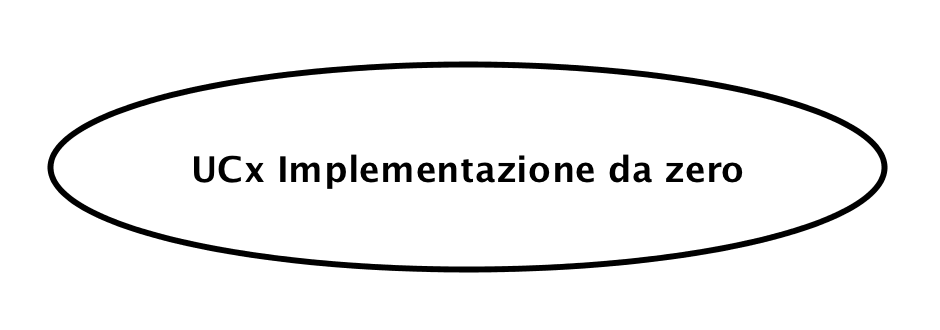
\includegraphics[width=7cm]{Pics/UCDaZero.png}
				\caption{Notazione di caso d'uso  relativo ad una componenti progettate da zero;}
				\label{fig:DiagrammaUCDaZero}
			\end{center}
		\end{figure}
		\item \textit{Caso d'uso relativo a componenti riprogettate dal punto di vista strutturale o dell'interfaccia utente:}
				 	\begin{figure}[H]
				 		\begin{center}
				 			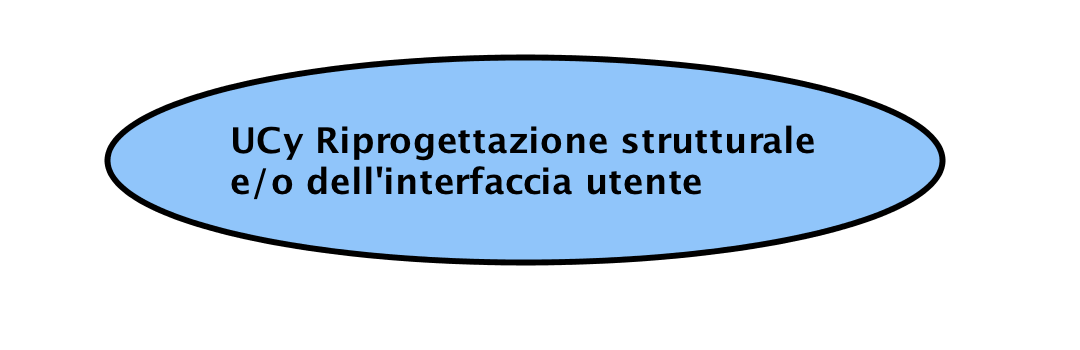
\includegraphics[width=8cm]{Pics/UCRestaurato.png}
				 			\caption{Notazione di caso d'uso relativo a componenti riprogettate.}
				 			\label{fig:DiagrammaUCRiprogettato}
				 		\end{center}
				 	\end{figure}		
	\end{itemize}
	\newpage
	\subsubsection{Attori}
	\begin{figure}[H]
		\begin{center}
			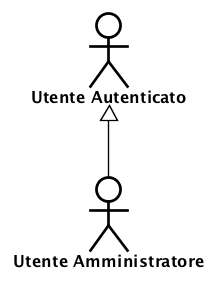
\includegraphics[width=5cm]{Pics/Attori.png}
			\caption{Attori coinvolti.}
			\label{fig:DiagrammaAttori}
		\end{center}
	\end{figure}	
	Sono state individuate due categorie di attori: 
	\begin{itemize}
		\item \texttt{Utente amministratore:} Utente che ha effettuato con successo il login nel sistema con privilegi da amministratore;
		\item \texttt{Utente autenticato:} Utente che ha effettuato con successo il login nel sistema.
	\end{itemize}
	
	L'\texttt{utente amministratore} specializza l'\texttt{utente autenticato}.
	
	\newpage
	\subsubsection{Caso d'uso UCP - Scenario Principale }
	\begin{figure}[H]
		\begin{center}
			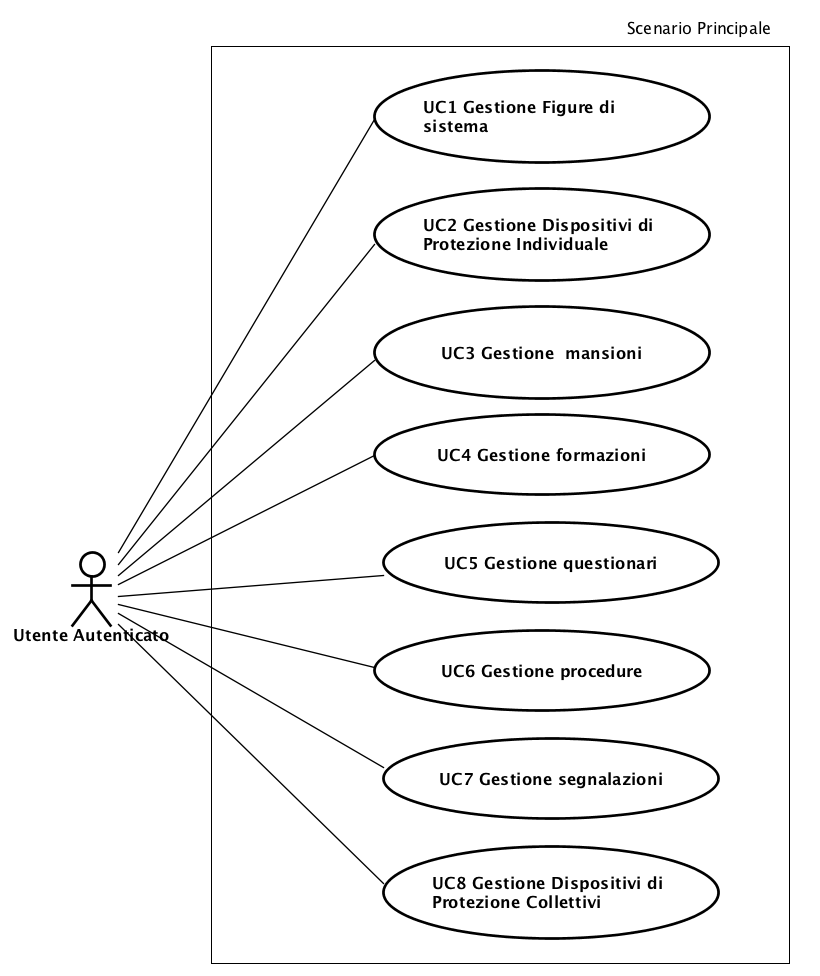
\includegraphics[width=11cm]{Pics/Diagramma_generale_dei_casi_d_uso.png}
			\caption{
				Diagramma dei casi d'uso generale.}
			\label{fig:DiagrammaGeneraleCasiDuso}
		\end{center}
	\end{figure}	
	
	\begin{itemize}
		\item \textbf{Scopo:} Il diagramma generale dei casi d'uso UCP (\autoref{fig:DiagrammaGeneraleCasiDuso}), ha lo scopo di rappresentare ad alto livello i casi d'uso necessari al soddisfacimento di tutti i requisiti. \\
		In particolare un utente che abbia effettuato con successo il login nel sistema, deve poter gestire: figure di sistema; dispositivi di protezione individuali, mansioni, formazioni, questionari, procedure; segnalazioni e dispositivi di protezione collettivi.
		A seguire la spiegazione e l'esplosione in sotto casi d'uso per ognuno dei casi d'uso sopra elencati.
		\item \textbf{Attori Coinvolti:} Utente Autenticato;
		\item \textbf{Flusso principale degli eventi:} 
			\begin{itemize}
				\item \textit{L'utente autenticato gestisce le Figure di sistema (\hyperref[section:UC1]{UC1});}
				\item \textit{L'utente autenticato gestisce i Dispositivi di Protezione Individuale (\hyperref[section:UC2]{UC2});}
				\item \textit{L'utente autenticato gestisce le mansioni (\hyperref[section:UC3]{UC3});}
				\item \textit{L'utente autenticato gestisce le formazioni (\hyperref[section:UC4]{UC4});}
				\item \textit{L'utente autenticato gestisce le procedure (\hyperref[section:UC5]{UC5});}
				\item \textit{L'utente autenticato gestisce le segnalazioni (\hyperref[section:UC6]{UC6})}
				\item \textit{L'utente autenticato gestisce i Dispositivi di Protezione Collettivi (\hyperref[section:UC7]{UC7}).}
			\end{itemize}
	\end{itemize}
	

	\subsubsection{UC1 Gestione delle Figure di sistema}
	\label{section:UC1}
	\begin{figure}[H]
		\begin{center}
			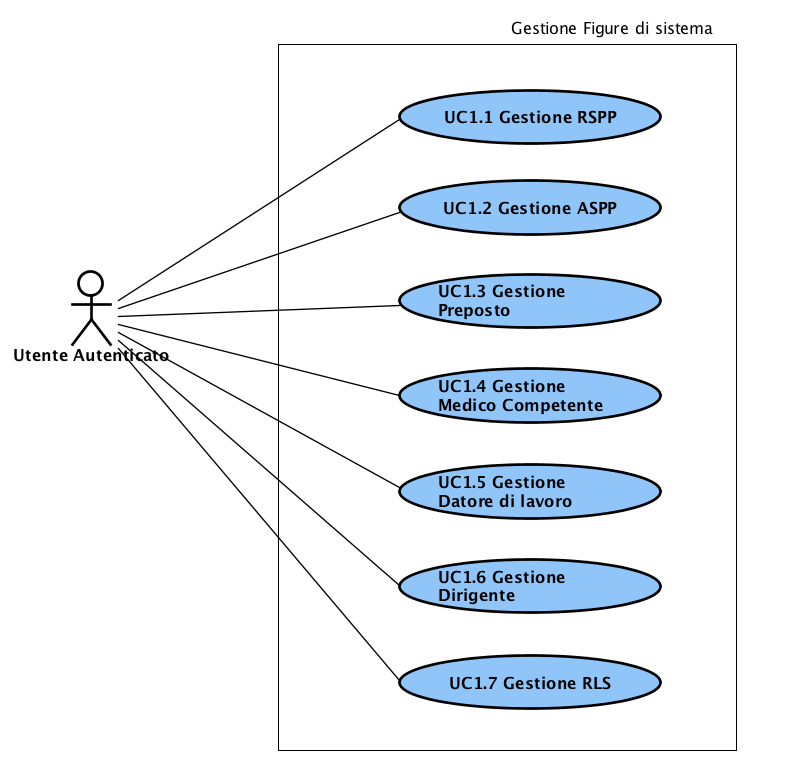
\includegraphics[width=12cm]{Pics/UC1GestioneFigureDiSistema.png}
			\caption{
				Diagramma dei casi d'uso UC1 - Figure di sistema.}
			\label{fig:UC1GestioneFigureDiSistema}
		\end{center}
	\end{figure}
	\begin{itemize}
		\item \textbf{Scopo:} Il diagramma generale dei casi d'uso UC1 (\autoref{fig:UC1GestioneFigureDiSistema}), ha lo scopo di rappresentare ad alto livello i casi d'uso necessari al soddisfacimento di tutti i requisiti rigruardanti le figure di sistema;
		\item \textbf{Attori Coinvolti:} Utente Autenticato;
		\item \textbf{Flusso principale degli eventi:} 
		\begin{itemize}
			\item \textit{L'utente autenticato gestisce gli \gls{RSPP}\G\ (\hyperref[section:UC1_1]{UC1.1});}
			\item \textit{L'utente autenticato gestisce gli \gls{ASPP}\G\ (UC1.2);}
			\item \textit{L'utente autenticato gestisce i preposti (UC1.3);}
			\item \textit{L'utente autenticato gestisce il medico competente (UC1.4);}
			\item \textit{L'utente autenticato gestisce il datore di lavoro (UC1.5);}
			\item \textit{L'utente autenticato gestisce i dirigenti (UC1.6);}
			\item \textit{L'utente autenticato gestisce gli \gls{RLS}\G\  (UC1.7).}
		\end{itemize}
	\end{itemize}
	
	\newpage
	\subsubsection{UC1.1 Gestione degli RSPP}
	\label{section:UC1_1}
	Tutte le figure di sistema presentano requisiti analoghi. Per evitare di affaticare la lettura con sezioni ridondanti è stato scelto di riportare soltanto il diagramma dei casi d'uso riguardante gli \gls{RSPP}\G. Si intende che per tutte le altre figure di sistema il diagramma sia analogo. 
		\begin{figure}[H]
			\begin{center}
				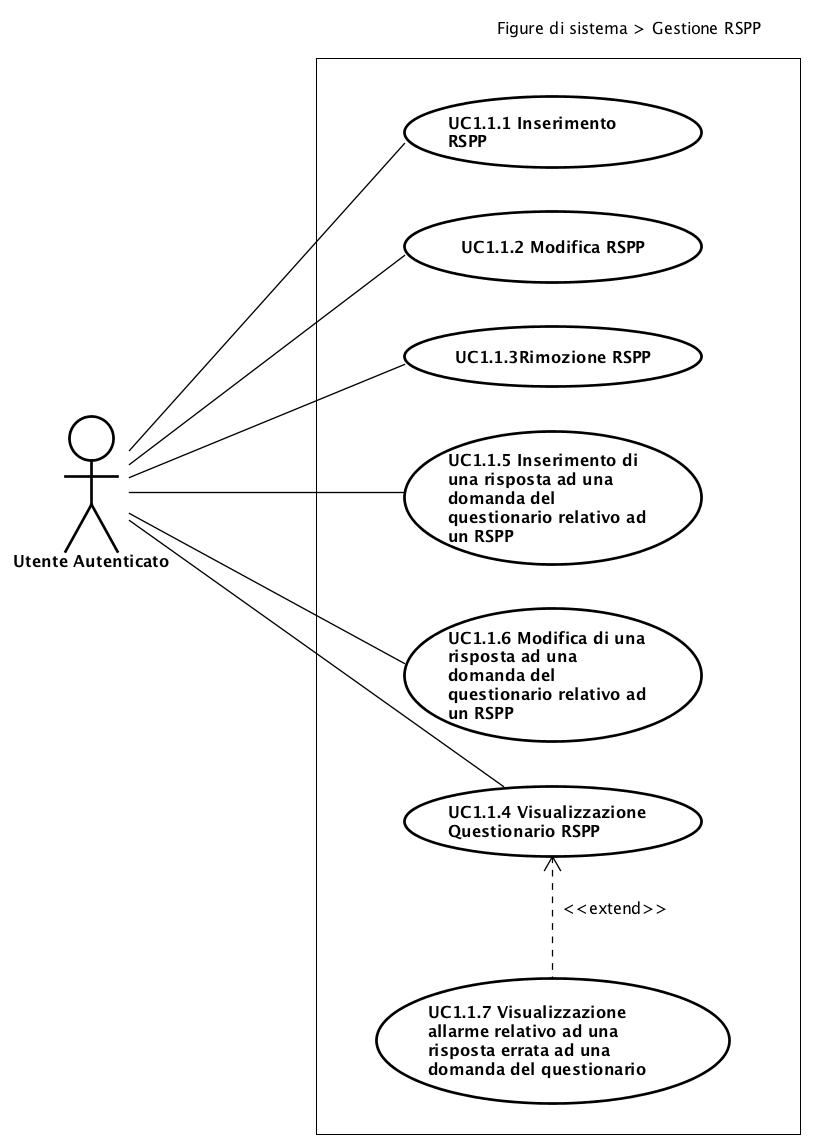
\includegraphics[width=12cm]{Pics/UC1_1_FigureDiSistema_RSPP.png}
				\caption{Diagramma dei casi d'uso relativo all'inserimento degli RSPP}
				\label{fig:UC1_1RSPP}
			\end{center}
		\end{figure}
		\begin{itemize}
			\item \textbf{Scopo:} Il diagramma relativo alla gestione degli RSPP (\autoref{fig:DiagrammaGeneraleCasiDuso}), ha lo scopo di rappresentare i casi d'uso necessari al soddisfacimento di tutti i requisiti riguardanti la gestione degli RSPP. \\
			In particolare un utente che abbia effettuato con successo il login nel sistema, deve poter inserire, rimuovere, modificare  \gls{RSPP}\G. Deve essere messo in condizione inoltre di Visualizzare un questionario relativo ad uno specifico \gls{RSPP}\G, rispondendo alle domande riportate su di esso. In caso di errore, deve essere sollevato un allarme che comunica la domanda esatta ed un messaggio esplicativo.
			\item \textbf{Attori Coinvolti:} Utente Autenticato;
			\item \textbf{Flusso principale degli eventi:} 
			\begin{itemize}
				\item \textit{L'utente autenticato inserisce un \gls{RSPP}\G\ (UC1.1.1);}
				\item \textit{L'utente autenticato modifica un \gls{RSPP}\G\ (UC1.1.2);}
				\item \textit{L'utente autenticato rimuove un \gls{RSPP}\G\  (UC1.1.3);}
				\item \textit{L'utente autenticato visualizza il questionario associato ad un \gls{RSPP}\G\  (UC1.1.4);}
				\item \textit{L'utente autenticato inserisce una risposta ad una domanda del questionario (UC1.1.5);}
				\item \textit{L'utente autenticato modifica di una risposta ad una domanda del questionario relativo ad un \gls{RSPP}\G\  (UC1.1.6);}
				\item \textit{ L'utente autenticato visualizza un allarme relativo ad una risposta errata ad una domanda del questionario (UC1.1.7).}
			\end{itemize}
		\end{itemize}
	\newpage	
	\subsubsection{UC2 Gestione dei DPI}
		\label{section:UC2}
		La gestione dei  \gls{DPI}\G\ va suddivisa in due scenari distinti. Il primo scenario è relativo alla gestione delle tipologie di \gls{DPI}\G\ disponibili da parte degli utenti amministratori. Il secondo scenario riguarda la gestione dei \gls{DPI}\G\ che compongono la dotazione personale di un dipendente. \\
		Seguono i diagrammi dei casi d'uso dei \gls{DPI}\G\ relativi agli scenari sopra indicati.

		\paragraph*{UC2.1 Gestione delle tipologie di DPI dal pannello di amministrazione }\mbox{} \\
			\label{section:UC2_1}
			\begin{figure}[H]
				\begin{center}
					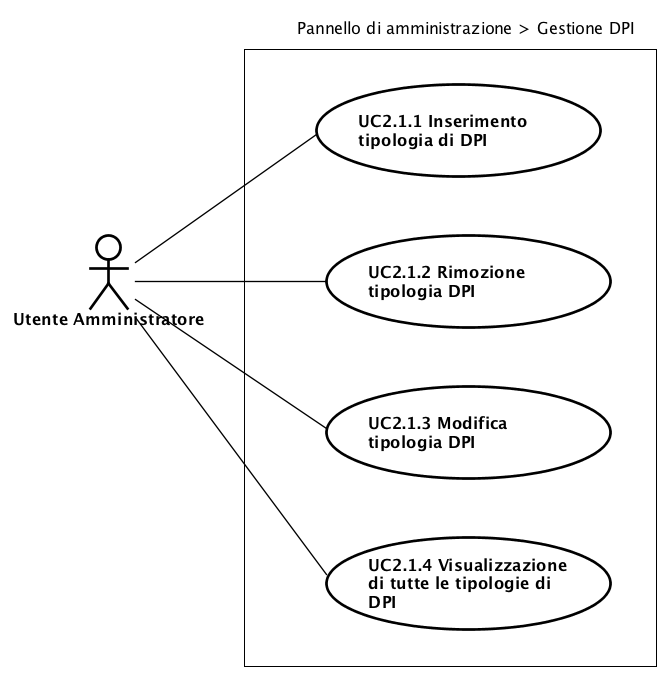
\includegraphics[width=12cm]{Pics/UC2_1GestioneDispositiviDiProtezioneIndividualeDaPannelloDiAmministrazione.png}
					\caption{
						Diagramma dei casi d'uso UC2.1 - Gestione tipologie di DPI dal pannello di amministrazione.}
					\label{fig:UC2_1GestioneDPIAmministrazione}
				\end{center}
			\end{figure}
			\begin{itemize}
				\item \textbf{Scopo:} Il diagramma presentato nella \autoref{fig:UC2_1GestioneDPIAmministrazione}, ha lo scopo di rappresentare i casi d'uso necessari al soddisfacimento di tutti i requisiti riguardanti la gestione delle tipologie dei \gls{DPI}\G.
				 \\ Un utente amministratore deve poter gestire in modo autonomo le tipologie di \gls{DPI}\G\ che ritiene più opportune e metterle a disposizione degli utilizzatori del sistema.
				\item \textbf{Attori Coinvolti:} Utente Amministratore;
				\item \textbf{Flusso principale degli eventi:} 
				\begin{itemize}
					\item \textit{L'utente amministratore inserisce una tipologia di \gls{DPI}\G\ (UC2.1.1);}
					\item \textit{L'utente amministratore rimuove una tipologia di \gls{DPI}\G\ (UC2.1.2);}
					\item \textit{L'utente amministratore modifica una tipologia di \gls{DPI}\G\ (UC2.1.3);}
					\item \textit{L'utente amministratore visualizza tutte le tipologie di \gls{DPI}\G\ (UC2.1.3).}
				\end{itemize}
			\end{itemize}
		\paragraph*{UC2.2 Gestione dei DPI assegnati ai dipendenti}\mbox{} \\
			\label{section:UC2_2}
			\begin{figure}[H]
				\begin{center}
					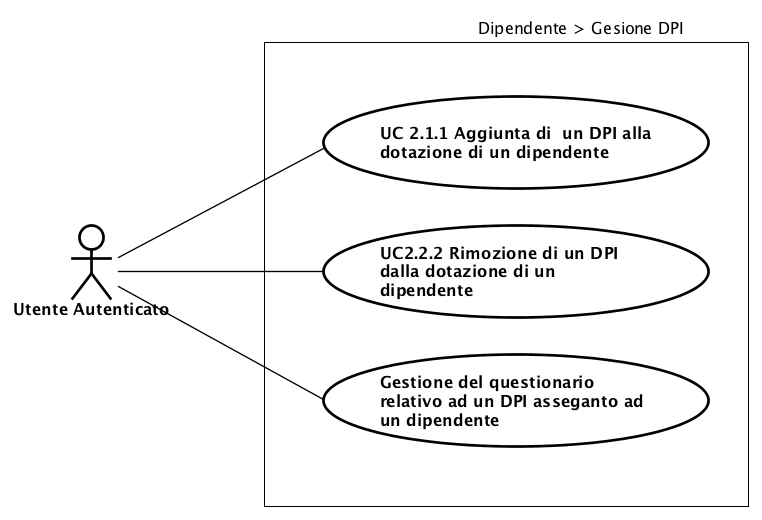
\includegraphics[width=12cm]{Pics/UC2_2DPIDipendenti.png}
					\caption{
						Diagramma dei casi d'uso UC2.2 - Gestione dei DPI relativi ad un dipendente.}
					\label{fig:UC2_2GestioneDPIDipendenti}
				\end{center}
			\end{figure}
			\begin{itemize}
				\item \textbf{Scopo:} Il diagramma presentato nella \autoref{fig:UC2_2GestioneDPIDipendenti}, ha lo scopo di rappresentare i casi d'uso necessari al soddisfacimento di tutti i requisiti riguardanti la gestione dei \gls{DPI}\G\ dati in dotazione ai dipendenti. \\ Un utente autenticato deve poter assegnare o rimuovere \gls{DPI}\G\ ad ogni dipendente. Deve essere possibile assegnare \gls{DPI}\G\ con molteplicità variabile, scegliendo la tipologia da una lista predefinita (Sezione: \ref{section:UC2_1}).\\
				Per ogni \gls{DPI}\G\ deve essere possibile rispondere ad un questionario;
				\item \textbf{Attori Coinvolti:} Utente Autenticato;
				\item \textbf{Flusso principale degli eventi:} 
				\begin{itemize}
					\item \textit{L'utente autenticato aggiunge un \gls{DPI}\G\ alla dotazione di un dipendente (UC2.2.1);}
					\item \textit{L'utente autenticato rimuove un \gls{DPI}\G\ dalla dotazione di un dipendente  (UC2.2.2);}
					\item \textit{L'utente autenticato gestisce il questionario relativo ad un \gls{DPI}\G\ assegnato ad un dipendente (UC2.2.3);}
					\item \textit{L'utente autenticato visualizza tutti i \gls{DPI}\G\ assegnati ad un dipendente (UC2.2.4).}
				\end{itemize}
			\end{itemize}
	
	\newpage		
	\subsubsection{UC3 Gestione  delle mansioni}
		\label{section:UC3}
		Le mansioni rappresentano le attività che un individuo interno all'azienda è abilitato a svolgere.\\
		L'associazione agli individui e la gestione delle mansioni disponibili è stato eseguito allo stesso modo dei \gls{DPI}\G. \\
		Per evitare di affaticare la lettura con sezioni ridondanti è stato scelto di riportare soltanto il diagramma dei casi d'uso riguardante i \gls{DPI}\G. Si intende che per le mansioni il diagramma e la spiegazione del caso d'uso sia analogo alla sezione \ref{section:UC2_2}.\\
		\newpage 
	\subsubsection{UC4 Gestione delle formazioni}
		\label{section:UC4}
		Con il termine formazione si intende una certificazione relativa ad un corso abilitante ad una o più mansioni.\\
		La gestione delle formazioni è del tutto simile a quella dei \gls{DPI}\G, fatta eccezione per la gestione delle scadenze. È richiesto infatti che un utente amministratore possa assegnare un periodo di validità della formazione in mesi dal pannello di controllo. Un utente autenticato deve visualizzare un allarme nel momento in cui una formazione sia scaduta.

	\paragraph*{UC4.1 Gestione delle formazioni dal pannello di amministrazione }\mbox{} \\
		\label{section:UC4_1}
		Tutte le considerazioni della sezione \ref{section:UC2} valgono anche per le formazioni. \\
		A differenza dei \gls{DPI}\G\ va inserita una informazione aggiuntiva obbligatoria: il periodo di validità della formazione. \\
		Il diagramma dei casi d'uso è del tutto analogo a quello della  \autoref{fig:UC2_1GestioneDPIAmministrazione}.
	\paragraph*{UC4.2 Gestione delle formazioni dei dipendenti e del datore di lavoro }\mbox{} \\
		\label{section:UC4_2}
		\begin{figure}[H]
			\begin{center}
				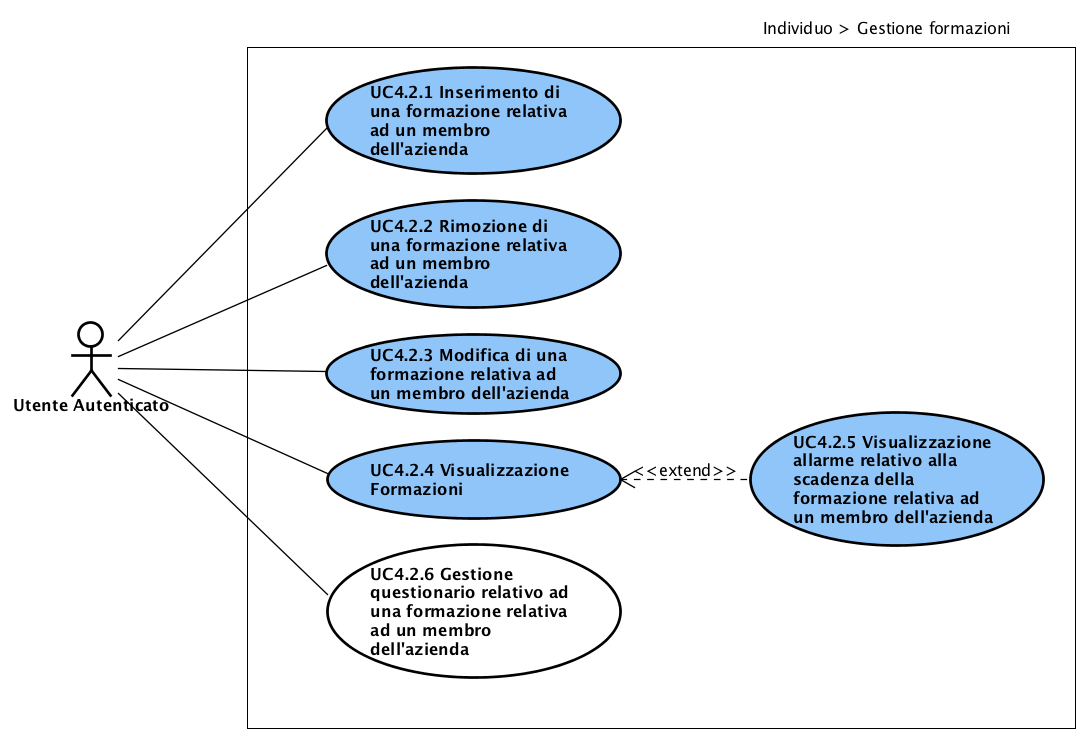
\includegraphics[width=16cm]{Pics/UC4_2GestioneFormazioni.png}
				\caption{Diagramma dei casi d'uso relativo alla gestione delle formazioni di un dipendente.}
				\label{fig:UC4_2_Formazioni}
			\end{center}
		\end{figure}
		
		\begin{itemize}
			\item \textbf{Scopo:} Il diagramma presentato nella \autoref{fig:UC4_2_Formazioni}, ha lo scopo di rappresentare i casi d'uso necessari al soddisfacimento di tutti i requisiti riguardanti la gestione delle formazioni relative ad un qualunque membro dell'azienda. \\ 
			Un utente autenticato deve poter assegnare o rimuovere formazioni ad ogni dipendente. 
			Ogni formazione relativa ad un dipendente deve essere dotata di un questionario. \\ 
			La scadenza della formazione deve essere segnalata trenta giorni prima della data ultima mediante un allarme.
			\item \textbf{Attori Coinvolti:} Utente Autenticato;
			\item \textbf{Flusso principale degli eventi:} 
			\begin{itemize}
				\item \textit{L'utente autenticato aggiunge una formazione ad un membro dell'azienda indicando descrizione e data (UC4.2.1);}
				\item \textit{L'utente autenticato rimuove una formazione ad un membro dell'azienda (UC4.2.2);}
				\item \textit{L'utente autenticato modifica una formazione ad un membro dell'azienda (UC4.2.3);}
				\item \textit{L'utente autenticato visualizza le formazioni relative ad un membro dell'azienda (UC4.2.4);}
				\item \textit{L'utente autenticato visualizza l'allarme relativo alla scadenza di una formazione in possesso di un membro dell'azienda (UC4.2.5);}
				\item \textit{L'utente autenticato gestisce il questionario relativo ad una formazione in possesso di un membro dell'azienda (UC4.2.6).}
			\end{itemize}
		\end{itemize}
	\newpage	
%	\subsubsection{UC5 Gestione dei questionari}
%	\hl{TODO Rimuovere e sistemare tutta la numerazione degli uc successivi + riferimenti nella tabella dei requisiti}
%	
%		\label{section:UC5}	
%			\begin{figure}[H]
%				\begin{center}
%					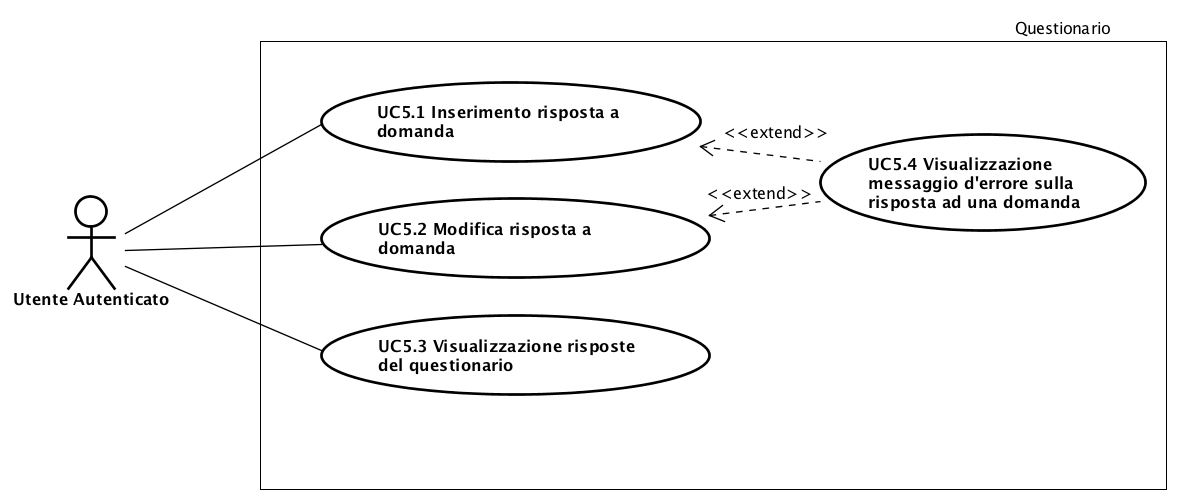
\includegraphics[width=15cm]{Pics/UC5QuestionarioUtenteAutenticato.png}
%					\caption{Diagramma dei casi d'uso relativo alla gestione di un questionario.}
%					\label{fig:UC5_Qestionari}
%				\end{center}
%			\end{figure}
%			
%			\begin{itemize}
%				\item \textbf{Scopo:} Il diagramma presentato nella \autoref{fig:UC5_Qestionari}, ha lo scopo di rappresentare i casi d'uso necessari al soddisfacimento dei requisiti riguardanti la gestione di un questionario di pertinenza di un utente autenticato. \\ 
%				Gli utenti amministratori devono poter gestire le domande poste nei questionari da un pannello d'amministrazione. Questo aspetto non è stato trattato in dettaglio poiché analogo a quanto descritto nella sezione \ref{section:UC2_1}.
%				\item \textbf{Attori Coinvolti:} Utente Autenticato;
%				\item \textbf{Flusso principale degli eventi:} 
%				\begin{itemize}
%					\item \textit{L'utente autenticato risponde per la prima volta ad una domanda (UC5.1);}
%					\begin{itemize}
%						\item \textit{Viene mostrato un messaggio d'errore se la risposta fornita non è corretta (UC5.4);}
%					\end{itemize}
%					\item \textit{L'utente autenticato modifica una risposta ad una domanda (UC5.2);}
%					\begin{itemize}
%						\item \textit{Viene mostrato un messaggio d'errore se la risposta fornita non è corretta (UC5.4);}
%					\end{itemize}
%					\item \textit{L'utente autenticato visualizza tutte le risposte al questionario (UC5.3). Se è la prima volta che lo apre, le risposte saranno tutte vuote.}
%				\end{itemize}
%			\end{itemize}
%


	\newpage		
	\subsubsection{UC5 Gestione delle procedure}
		\label{section:UC5}
		Le procedure rappresentano un aspetto di primaria importanza e si suddividono in due categorie: di prassi e di sistema. \\
		Le procedure di prassi derivano direttamente da un documento fornito dall'\gls{INAIL}\G. Queste procedure sono state individuate dall'analisi delle cause di infortunio maggiormente frequenti rilevate dall'\gls{INAIL}\G\ nel tempo allo scopo di migliorare la sicurezza dei lavoratori.
		Le procedure di sistema, invece, sono stese dall'azienda e fanno parte del \gls{DVR}\G. 
		\begin{figure}[H]
			\begin{center}
				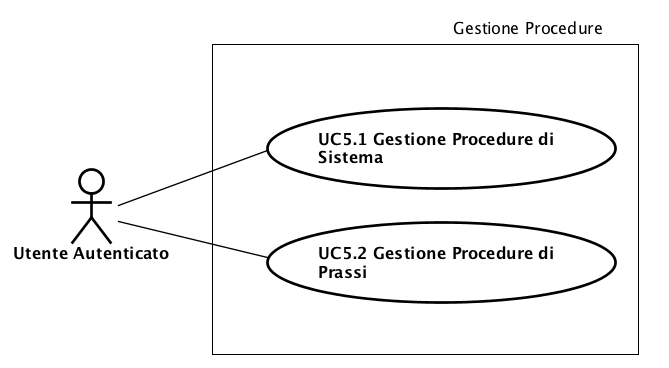
\includegraphics[width=12cm]{Pics/UC5GestioneProcedure.png}
				\caption{Diagramma dei casi d'uso relativo alla gestione delle procedure.}
				\label{fig:UC5_Procedure}
			\end{center}
		\end{figure}
		
			\begin{itemize}
				\item \textbf{Scopo:} Il diagramma presentato nella \autoref{fig:UC5_Procedure}, ha lo scopo di rappresentare i casi d'uso necessari alla gestione delle procedure all'interno dell'azienda. \\ 
				
				Un utente autenticato deve poter gestire le procedure di ogni dipendente dell'azienda. \\
				Ogni procedura, di sistema, deve essere dotata di descrizione, codifica ed informazioni relative alle revisioni delle quali è stata oggetto nel tempo.\\
				Le procedure di prassi sono state gestite con un questionario in quanto derivanti direttamente da una lista di domande proveniente dall'\gls{INAIL}\G;
				\item \textbf{Attori Coinvolti:} Utente Autenticato;
				\item \textbf{Flusso principale degli eventi:} 
				\begin{itemize}
					\item \textit{L'utente autenticato gestisce le procedure di sistema(UC5.1);}
					\begin{itemize}
						\item \textit{L'utente autenticato inserisce una nuova procedura di sistema(UC5.1.1);}
						\item \textit{L'utente autenticato modifica una procedura di sistema(UC5.1.2);}
						\item \textit{L'utente autenticato rimuove una procedura di sistema(UC5.1.3);}
						\item \textit{L'utente autenticato visualizza tutte le procedure di sistema(UC5.1.4).}
					\end{itemize}
					\item \textit{L'utente autenticato gestisce le procedure di prassi (UC5.2);}
					\begin{itemize}
						\item \textit{L'utente autenticato inserisce una nuova procedura di prassi (UC5.2.1);}
						\item \textit{L'utente autenticato modifica una procedura di prassi (UC5.2.2);}
						\item \textit{L'utente autenticato rimuove una procedura di prassi (UC5.2.3);}
						\item \textit{L'utente autenticato visualizza tutte le procedure di prassi (UC5.2.4).}
					\end{itemize}
				\end{itemize}
			\end{itemize}
			
	\newpage
	\subsubsection{UC6 Gestione delle segnalazioni}
		\label{section:UC6}	
		Le segnalazioni sono delle comunicazioni ufficiali indirizzate all'organo di vigilanza. Esse sono dotate di: descrizione, segnalante, data di comunicazione del segnalante all'alta direzione, data di comunicazione dall'alta direzione all'organo di vigilanza, data di risposta dell'organo di vigilanza al soggetto interessato.\\
		\begin{figure}[H]
			\begin{center}
				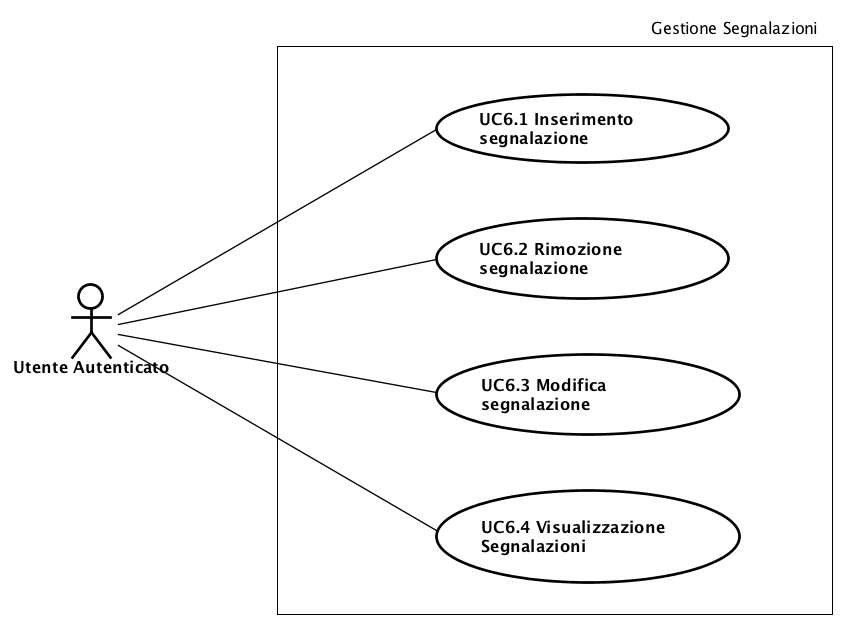
\includegraphics[width=12cm]{Pics/UC6Segnalazioni.png}
				\caption{Diagramma dei casi d'uso relativo alla gestione delle segnalazioni.}
				\label{fig:UC6_Segnalazioni}
			\end{center}
		\end{figure}
		
		\begin{itemize}
			\item \textbf{Scopo:} Il diagramma presentato nella \autoref{fig:UC6_Segnalazioni}, ha lo scopo di rappresentare i casi d'uso necessari al soddisfacimento di tutti i requisiti riguardanti la gestione delle segnalazioni all'interno dell'azienda. \\ 
			\item \textbf{Attori Coinvolti:} Utente Autenticato;
			\item \textbf{Flusso principale degli eventi:} 
			\begin{itemize}
				\item \textit{L'utente autenticato inserisce una segnalazione (UC6.1);}
				\item \textit{L'utente autenticato rimuove una segnalazione (UC6.2);}
				\item \textit{L'utente autenticato modifica una segnalazione (UC6.3);}
				\item \textit{L'utente autenticato visualizza tutte le segnalazioni (UC6.4);}
			\end{itemize}
		\end{itemize}
		
	\newpage	
	\subsubsection{UC7 Gestione dei Dispositivi di Protezione Collettivi}
		\label{section:UC7}
		\begin{figure}[H]
			\begin{center}
				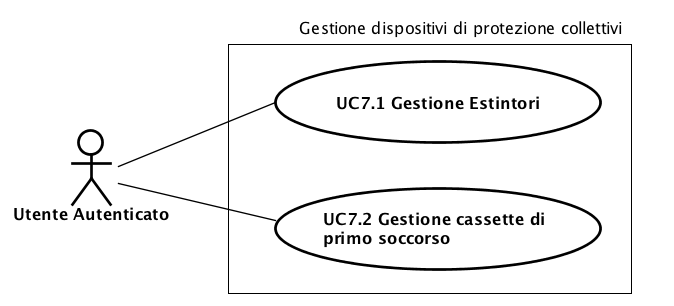
\includegraphics[width=12cm]{Pics/UC7GestioneDispositiviProtezioneCollettivi.png}
				\caption{Diagramma dei casi d'uso relativo alla gestione dei Dispositivi di Protezione Collettiva (DPC).}
				\label{fig:UC7_DPC}
			\end{center}
		\end{figure}
		
		\begin{itemize}
			\item \textbf{Scopo:} Il diagramma presentato nella \autoref{fig:UC7_DPC}, ha lo scopo di rappresentare i casi d'uso necessari al soddisfacimento di tutti i requisiti riguardanti la gestione dei \gls{DPC}\G\ all'interno dell'azienda. \\ 
			\item \textbf{Attori Coinvolti:} Utente Autenticato;
			\item \textbf{Flusso principale degli eventi:} 
			\begin{itemize}
				\item \textit{L'utente autenticato gestisce gli estintori(UC7.1);}
				\begin{itemize}
					\item \textit{L'utente autenticato inserisce un nuovo estintore (UC7.1.1);}
					\item \textit{L'utente autenticato modifica un estintore(UC7.1.2);}
					\item \textit{L'utente autenticato rimuove un estintore (UC7.1.3);}
					\item \textit{L'utente autenticato visualizza tutti gli estintori (UC7.1.4).}
				\end{itemize}
				\item \textit{L'utente autenticato gestisce le cassette di primo soccorso (UC7.2);}
				\begin{itemize}
					\item \textit{L'utente autenticato inserisce una nuova cassetta di primo soccorso (UC7.2.1);}
					\item \textit{L'utente autenticato modifica una cassetta di primo soccorso (UC7.2.2);}
					\item \textit{L'utente autenticato rimuove una cassetta di primo soccorso (UC7.2.3);}
					\item \textit{L'utente autenticato visualizza tutte le cassette di primo soccorso (UC7.2.4).}
				\end{itemize}
			\end{itemize}
		\end{itemize}

\newpage

\subsection{Requisiti}
Al fine di chiarire ciò che si è svolto durante lo stage, è riportata la seguente tabella relativa ai requisiti che devono essere soddisfatti.\\
I requisiti sono stati stesi sulla base di diversi colloqui con il committente e da vincoli interni all'azienda. Dopo ogni  colloquio, è stato steso il relativo verbale.\\ Tutti i requisiti provenienti dai verbali che fanno seguito ai colloqui sono stati catalogati come fonte interna.\\
La codifica di ogni requisito è così composta:
\begin{itemize}
	\item Una \textit{R} iniziale per sottolineare il fatto che si tratta di un requisito;
	\item Un qualificatore del livello di importanza:
	\begin{itemize}
		\item \textit{obb}: obbligatorio;
		\item \textit{des}: desiderabile;
		\item \textit{opz}: opzionale.
	\end{itemize}
	\item Un qualificatore relativo alla tipologia:
	\begin{itemize}
		\item \textit{F}: funzionale;
		\item \textit{Q}: qualitativo;
		\item \textit{V}: vincolo.
	\end{itemize}
	\item Un numero progressivo.
\end{itemize}

\newcolumntype{l}[1]{m{#1}}
\begin{flushleft}
	\begin{tabular}{|l{2cm}|l{8cm}|l{2cm}|}

		\hline
		\textbf{Codice} & \textbf{Descrizione} & \textbf{Fonti} \\
		\hline
		%vincoli
		\label{RobbV0}
		\textit{RobbV0} & Il codice deve essere scritto utilizzando Ruby on Rails. & Azienda \\
		\hline
		%FIGURE DI SISTEMA
		\label{RobbF0}
		\textit{RobbF0} & Un dipendente deve poter ricoprire più cariche contemporaneamente. & fonte interna, \hyperref[section:UC1]{UC1}\\
		\hline
		\label{RdesF1}
		\textit{RobbF1} & Un dipendente deve poter ricoprire una carica in un dato luogo. & fonte interna, \hyperref[section:UC1]{UC1}\\
		\hline
		\label{RobbF1.1}
		\textit{RobbF1.1} & Per ogni carica di ogni dipendente devono essere gestite le informazioni relative alla nomina. & fonte interna, \hyperref[section:UC1]{UC1},\\
		\hline
		\label{RobbF1.2}
		\textit{RobbF1.2} & Per ogni carica di ogni dipendente devono essere segnalate eventuali formazioni mancanti per poterla ricoprire. & fonte interna, \hyperref[section:UC1]{UC1}\\
		\hline
		\label{RobbF1.3}
		\textit{RobbF1.3} & Un \gls{ASPP}\G\ oppure un \gls{RSPP}\G\ deve poter essere sia un membro interno sia esterno all'azienda. & fonte interna, \hyperref[section:UC1]{UC1}, \hyperref[section:UC1_1]{UC1.1} \\
		\hline
		\label{RobbF1.4}
		\textit{RobbF1.4} & Tutte le informazioni relative alle \textit{figure di sitema} devono essere gestibili in un unica sezione. & fonte interna\\
		\hline
		%DPI
		\label{RobbF2}
		\textit{RobbF2} & Un utente amministratore deve poter gestire le tipologie di \gls{DPI}\G\ messe a disposizione dal sistema. & fonte interna, \hyperref[section:UC2_1]{UC2.1}\\
		\hline
		\label{RobbF2.1}
		\textit{RobbF2.1} & Un utente autenticato deve poter aggiungere un \gls{DPI}\G\ alla dotazione di un dipendente  selezionandolo esclusivamente tra quelli messi a disposizione da \hyperref[RobbF2]{RobbF2}. &  \hyperref[section:UC2_1]{UC2.2.1}\\
		\hline
		\label{RobbF2.2}
		\textit{RobbF2.2} & Un utente autenticato deve poter inserire le informazioni aggiuntive relative ad ogni \gls{DPI}\G\ di ogni dipendente. & fonte interna, \hyperref[section:UC2_2]{UC2.2.3}\\
		\hline
		\label{RdesF2.3}
		\textit{RdesF2.3} & La scadenza di un \gls{DPI}\G\ deve essere segnalata con trenta giorni di preavviso. & fonte interna \\
		\hline
		%MANSIONI
		\label{RobbF3}
		\textit{RobbF3} & Un utente amministratore deve poter gestire le denominazioni delle mansioni messe a disposizione dal sistema. & UC3.1\\
		\hline
		\label{RobbF3.1}
		\textit{RobbF3.1} & Un utente autenticato deve poter assegnare una mansione ad un dipendente selezionandola esclusivamente tra le denominazioni messe a disposizione da \hyperref[RobbF3]{RobbF3}. & UC3.2.1 \\
		\hline
		\label{RobbF3.2}
		\textit{RobbF3.2} & Un utente autenticato deve poter inserire le informazioni aggiuntive relative ad ogni mansione assegnata ad ogni dipendente. & UC3.2.3\\
		\hline
	\end{tabular}
\end{flushleft}
\newpage

\begin{flushleft}
	\begin{tabular}{|l{2cm}|l{8cm}|l{2cm}|}
		\hline
		\textbf{Codice} & \textbf{Descrizione} & \textbf{Fonti} \\
		\hline
		%FORMAZIONI
		\label{RobbF4}
		\textit{RobbF4} & Un utente amministratore deve poter gestire le denominazioni delle formazioni messe a disposizione dal sistema. &  fonte interna, \hyperref[section:UC4_1]{UC4.1}\\
		\hline
		\label{RobbF4.1}
		\textit{RobbF4.1} & Un utente autenticato deve poter inserire una formazione di un dipendente selezionandola esclusivamente tra le denominazioni messe a disposizione da \hyperref[RobbF4]{RobbF4}. &  fonte interna, UC4.2.1 \\
		\hline
		\label{RobbF4.2}
		\textit{RobbF4.2} & Un utente autenticato deve poter inserire le informazioni aggiuntive relative ad ogni formazione conseguita da ogni dipendente. & fonte interna, UC3.2.3\\
		\hline
		% soddisfatto
		\label{RdesF4.3}
		\textit{RdesF4.3} & Un utente amministratore deve poter inserire le formazioni necessarie allo svolgimento di una data mansione. & fonte interna \\
		\hline
		%non soddisfatto
		\label{RdesF4.4}
		\textit{RdesF4.4} & La mancanza delle formazioni necessarie per poter svolgere una mansione deve essere segnalata. & fonte interna \\
		\hline
		\label{RobbQ5}
		\textit{RdesQ5} & Deve essere previsto un aiuto all'utente nella compilazione di un  questionario con una quantità rilevante di domande. & Azienda \\
		\hline
		\label{RobbF6}
		\textit{RobbF6} & Devono essere gestite in una apposita sezione le procedure aziendali che compongono il \gls{DVR}\G. & fonte interna, \hyperref[section:UC5]{UC5}\\
		\hline
		\label{RobbF6.1}
		\textit{RobbF6.1} & Devono essere poste tutte le domande che compongono le procedure di prassi fornite dall'\gls{INAIL}\ agli asseveratori. &  fonte interna, \hyperref[section:UC5]{UC5}\\
		\hline
		\label{RdesF7}
		\textit{RobbF7} & Un utente autenticato deve poter gestire le segnalazioni all'organo di vigilanza. & fonte interna,  \hyperref[section:UC6]{UC6}\\
		\hline
		\label{RobbF8}
		\textit{RobbF8} & Deve essere possibile gestire i  \gls{DPC} aziendali indicati in estintori e cassette di primo soccorso. & fonte interna, \hyperref[section:UC7]{UC7}\\
		\hline
		\label{RobbF8.1}
		\textit{RobbF8.1} & Deve essere possibile associare un \gls{DPC} ad una sede o ad un cantiere. & fonte interna\\
		\hline
		\label{RobbF9}
		\textit{RobbF9} & Deve essere possibile impostare regole di validazione delle informazioni inserite condizionata dal valore o la presenza di altre . & fonte interna\\
		\hline
		\label{RdesQ9.1}
		\textit{RopzQ9.1} & Devono essere disponibili degli script che caricano le informazioni minime funzionali all'installazione del sistema. & fonte interna\\
		\hline
		\label{RdesF9.2}
		\textit{RopzF9.2} & Un utente amministratore deve poter impostare regole di validazione da un editor \gls{WYSIWYG} . & Azienda \\
		\hline
		\label{RdesQ10}
		\textit{RdesQ10} & Stesura della documentazione relativa al codice prodotto. & Azienda \\
		\hline
	\end{tabular}
\end{flushleft}

	\cleardoublepage
	\section{Tecnologie e strumenti}
\subsection{Git}

Git è un sistema di controllo di versione sviluppato per facilitare la cooperazione nello sviluppo di software. Questo software di versionamento è gratuito ed open-source;  è stato sritto  da \textit{Linus Torvalds} per lo sviluppo del kernel linux nel 2005 ed attualmente mantenuto da \textit{Junio Hamano}. \\
\hl{TODO Aggiungere riferimento bibliografico}
Questo strumento permette di sottomettere al server le modifiche e lasciare ad esso l'onere di verificare se la versione appena inoltrata va in conflitto con quella esistente indicando esattamente in quale punto si è presentato il problema. \\
Viene data la possibilità di generare diversi rami (\textit{branch}) con l'intento di differenziare una nuova versione del codice (\textit{fork}) o per lo sviluppo di una nuova funzionalità, mentre nel primo caso il ramo diverge dal ramo da quale ha origine, nel secondo caso il \textit{branch} ha come fine il ricongiungimento con la sorgente da cui proviene una volta soddisfatto il suo contratto. È proprio da questa idea che nasce il concetto di \texttt{git-flow}.

\subsubsection{\texttt{git-flow}}
\begin{figure}[H]
\begin{center}
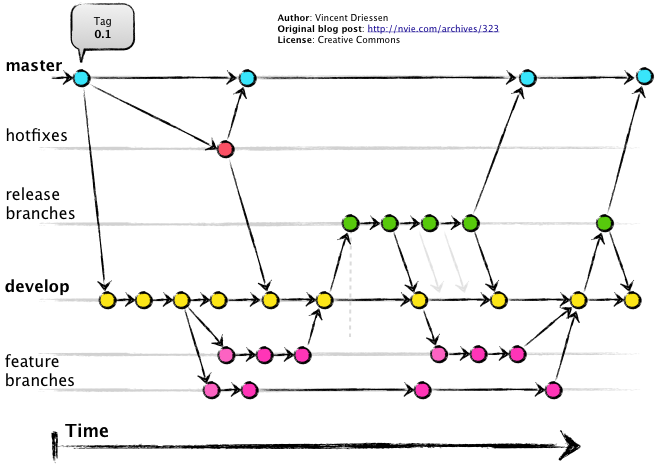
\includegraphics[width=12cm]{Pics/gitflow.png}
\caption{Grafico dei branch di \texttt{git-flow}}
\label{fig:GitFlow}
\end{center}
\end{figure}
Git-flow è un set di estensioni di git che offre dei comandi di alto livello sul repository per utilizzare il modello di branching (vedi \autoref{fig:GitFlow}) di \textit{Vincent Driessen}, fornendo il supporto a branching e release management.
Esso prevede due branch principali:
\begin{itemize}
\item \texttt{"master"}: ramo contenente il codice pronto per essere inoltrato nell'ambiente di produzione;
\item \texttt{"develop"}: ramo di riferimento per l'attività di sviluppo.
\end{itemize}
Sono previste inoltre altre tre tipologie di branch:
\begin{itemize}
\item \texttt{feature}: questo tipo di branch viene creato a partire dal ramo principale \texttt{develop}; dopo aver portato a compimento una particolare funzionalità, il branch \texttt{feature} viene fuso con lo stesso \texttt{develop};
\item \texttt{release}: questo branch è dedicato alla preparazione di un prodotto alla release; qui è possibile effettuare solo piccoli interventi di rimozione di bug (minor bugfix) in vista di un imminente rilascio nel branch master simultaneamente alla pubblicazione della nuova versione con il comando \texttt{git tag};
\item \texttt{hotfix}: questo ramo ha lo scopo di risolvere velocemente eventuali bug riscontrati; ha sempre origine dal branch master e, andando a modificare del software già rilasciato, provoca un avanzamento di sul numero di versione.
\end{itemize}
\paragraph{Vantaggi} 
\begin{itemize}
	\item Permette di mantenere una storia chiara e concisa del progetto poiché tutti i commit parziali avvengono nei branch di tipo feature.  Nel ramo develop, saranno presenti solo commit derivanti dalla fusione di rami di tipo feature che soddisfano pienamente il contratto per i quali sono stati creati;
	\item Evita di creare confusione nel repository con commit parziali potenzialmente dannosi e, dualmente, evitare le situazioni in cui lo sviluppo avviene localmente con un solo commit di grosse dimensioni al compimento del contratto del requisito perdendo i vantaggi dello storico dei commit offerti da git.
\end{itemize}
\paragraph{Svantaggi}
\begin{itemize}
	\item L'utilizzo di git-flow richiede agli sviluppatori di dedicare del tempo in più rispetto al metodo classico. Questo però è vero solo per progetti di piccole dimensioni poiché, al crescere dei progetti, il tempo impiegato a risolvere i conflitti derivanti dall'operare in modo classico risulta superiore a quello dedicato ad un corretto utilizzo di git-flow.
	\item Un ulteriore svantaggio è dato dal fatto che gli strumenti offerti dagli IDE per la gestione di git-flow non sono sempre all'altezza del loro compito.
\end{itemize}

\subsection{Rubymine}

\begin{figure}[H]
\begin{center}

\includegraphics[width=4cm]{Pics/rubymine_logo.png}
\caption{Logo di RubyMine}
\label{fig:RubyMine}
\end{center}
\end{figure}
Rubymine è un IDE prodotto da jetBrains, disegnato appositamente per lo sviluppo con Ruby on Rails.
\paragraph{Vantaggi}
\begin{itemize}
	\item Vengono messi a disposizione molti plugin gratuiti che offrono funzionalità specifiche, non incluse nel pacchetto base;
	\item Il salvataggio di un file avviene automaticamente ogni volta che esso perde il focus, dando la garanzia di lavorare sempre con file aggiornati;
	\item Il software è strutturato in modo tale da fornire aiuto attivo nel momento della stesura del codice, come autompletamento ed analisi statica, rendendo più veloce ed efficace il lavoro.
\end{itemize}
\paragraph{Svantaggi}
\begin{itemize}
	\item Il plugin responsabile del versionamento non funziona sempre alla perfezione, in particolare quando si utilizza git-flow.
\end{itemize}

\subsection{Ruby on Rails}

Ruby on Rails, è un framework open source per lo sviluppo di applicazioni web.
La sua architettura si basa sul pattern Model-View-Controller (MVC), realizzando a tutti gli effetti un framework full-stack; è dunque possibile realizzare sia la parte di backend che quella di \gls{front-end}\G.
\paragraph{Vantaggi}
\begin{itemize}
	\item Risorse e componenti sono integrati in modo tale che i collegamenti non debbano mai essere impostati manualmente, ma in modo automatico;
	\item È possibile lavorare utilizzando ActiveRecord, descritto nella sezione \ref{sec:ActiveRecord}. Questo è un grosso vantaggio perché velocizza la stesura del codice e risponde bene ai cambiamenti. Nel progetto svolto, l'utilizzo di ActiveRecord è un fattore determinante poiché è necessario che il software sia sempre conforme alle normative vigenti che cambiano nel tempo;
	\item È possibile disaccoppiare il backend ed il \gls{front-end}\G\ perché in Rails il routing delle risorse è gestito con una interfaccia \gls{REST}\G;
	\item Sono inoltre messi a disposizione i seguenti ambienti per uno stesso software, al fine di creare una separazione nel progetto:
		\begin{itemize}
		\item development 
		\item test
		\item production
		\end{itemize} 
		Ambienti distinti solitamente risiedono anche su server distinti.
	\item Sono presenti infine numerose librerie dette \textit{Gemme}, che offrono molteplici funzionalità velocizzando il lavoro.
\end{itemize}
\paragraph{Svantaggi}
	\begin{itemize}
		\item Ruby on Rails è meno performante rispetto ad altri linguaggi, ad esempio Java o Scala, ma di un ordine di grandezza non influente su progetti di medie dimensioni. 
	\end{itemize} 
		
\subsubsection{ActiveRecord}

\label{sec:ActiveRecord}
Active Record è il modulo di Ruby on Rails che gestisce la persistenza dei dati seguendo il pattern \textit{Active Record }di   %\cite{martinfowler:activerecord} .
Martin Fowler\footnote{La spiegazione dettagliata del pattern Active Record di Martin Fowler è descritta all'indirizzo \url{http://www.martinfowler.com/eaaCatalog/activeRecord.html}. }. \\
Il modulo ActiveRecord di Rails si serve di un database e prevede:
\begin{itemize}
\item Ogni tabella del database relazionale è gestita attraverso una classe;
\item Una singola istanza della classe corrisponde ad una riga (record) nella tabella associata;
\item Alla creazione di una nuova istanza viene creata una nuova riga all'interno della tabella che viene aggiornata ad ogni modifica dell'istanza associata.
\end{itemize}
Le colonne della tabella rappresentano gli attributi della classe.

\paragraph{Vantaggi} 
\begin{itemize}
	\item È possibile associare un diverso database per ogni ambiente predisposto da Rails separando i record memorizzati per lo sviluppo, per i test, o per l'ambiente di produzione;
	\item È disponibile un meccanismo di gestione delle relazioni molto efficiente che facilita dichiarazione ed utilizzo delle diverse tipologie di relazione tra le tabelle del database;
	\item Viene messo a disposizione un meccanismo specifico per la gestione dell'evoluzione dello schema del database mediante le \texttt{migrazioni} (vedi \autoref{App:AppendiceMigrazioni}). 
\end{itemize} 
\paragraph{Svantaggi}
\begin{itemize}
	\item Richiede una progettazione spesso diversa da quella classica, poiché l'ereditarietà risulta molto più difficile da gestire quando una classe corrisponde ad una tabella;
	\item Ad ogni migrazione, è necessario pensare bene a tutti gli effetti collaterali che potrebbero avvenire sugli statement che utilizzano la tabella modificata.
\end{itemize} 

\subsubsection{ActiveAdmin}

\begin{figure}[H]
\begin{center}

\includegraphics[width=6cm]{Pics/ActiveAdmin_logo.png}
\caption{Logo di ActiveAdmin}
\label{fig:ActiveAdminLogo}
\end{center}
\end{figure}
ActiveAdmin è una libreria (Gemma) di Ruby on Rails che permette di creare un sistema di amministrazione (backoffice). Mediante un pannello di gestione, permette di inserire, eliminare ed aggiornare istanze di modelli e relazioni direttamente da browser. 
\paragraph{Vantaggi}
\begin{itemize}
	\item Questa libreria permette ad un utente del sito di essere autonomo nell'aggiornamento dei contenuti senza dover attendere i tempi tecnici dell'azienda fornitrice;
	\item È fortemente personalizzabile, per questo è spesso utilizzato per la creazione di Dashboard o altre funzionalità dedicate ad utenti ai quali sono assegnati particolari privilegi d'accesso.
\end{itemize}
\paragraph{Svantaggi}
\begin{itemize}
	\item La grafica di ActiveAdmin risulta datata, è quindi spesso necessario riprogettare la veste grafica del pannello di amministrazione fornito di default.
\end{itemize}
\subsubsection{I18n}
	\begin{figure}[H]
		\begin{center}
			
\includegraphics[width=4cm]{Pics/i8n-logo.png}
			\caption{Logo di I18n}
			\label{fig:I18NLogo}
		\end{center}
	\end{figure}
	I18n è l'abbreviazione della parola "internationalization", deriva dal suo spelling che interpone 18 lettere tra la "i" iniziale e la "n" finale. \\ 
	Lo scopo è gestire la distribuzione del software in diverse lingue. Il meccanismo prevede un codice identificativo per ogni stringa da visualizzare, che assumerà un diverso valore per ogni traduzione. \\
	In Ruby, esiste una apposita gemma, denominata appunto \textit{I18N}, che fornisce le direttive per adottare correttamente questo approccio. \\
	Spesso il concetto di internazionalizzazione, viene associato a quello di localizzazione che è l'insieme dei processi di adattamento di un software , pensato e progettato per un mercato e contesto predefinito, in modo specifico ad altre nazione e culture. \\
	Tutte le informazioni di pertinenza di una lingua sono raccolti in un gruppo di parametri chiamato \textit{locale}.
\paragraph{Vantaggi}
	\begin{itemize}
		\item Grazie alla gemma \textit{i18n} , è possibile riutilizzare il codice responsabile della logica di business dell'applicazione e localizzare le stringhe per ogni lingua;
		\item L'aggiunta di nuove lingue richiede solo lo sforzo riguardante la traduzione ed eventuali conversioni nelle unità di misura appropriate;
		\item È possibile riutilizzare in contesti diversi le stringhe già definite, evitando quindi di introdurre errori di battitura;
		\item L'aggiunta di nuove lingue non provoca alcuna modifica nell'applicazione esistente, ma solo l'aggiunta del file in formato \texttt{yml} con le traduzioni.
	\end{itemize}
\paragraph{Svantaggi}
	\begin{itemize}
		\item La scrittura di codice con questo approccio richiede generalmente più tempo se il software esiste in una sola lingua.
	\end{itemize}
\subsection{JRuby}
	\begin{figure}[H]
		\begin{center}
			
\includegraphics[width=4cm]{Pics/jruby-logo.png}
			\caption{Logo di JRuby}
			\label{fig:JRubyLogo}
		\end{center}
	\end{figure}
	JRuby è un'implementazione in Java del linguaggio di programmazione Ruby. \\
	Sebbene non siano coperte tutte le implementazioni delle librerie standard offerte da Ruby, è comunque possibile utilizzare tutti la maggior parte delle funzionalità del  linguaggio.
\paragraph{Vantaggi}
\begin{itemize}
	\item JRuby è un software completamente gratuito;
	\item Gira su una JVM, quindi è possibile integrare l'interprete Ruby in una applicazione Java ed, allo stesso tempo, scrivere direttamente codice Java.
\end{itemize}
\paragraph{Svantaggi}
	\begin{itemize}
		\item È possibile incontrare situazioni in cui si necessita di una libreria che non è stata implementata;
		\item L'utilizzo di JRuby provoca un significativo appesantimento del software ed un conseguente peggioramento delle performance. 
	\end{itemize}
\subsection{Drools}
	\begin{figure}[H]
		\begin{center}
			
\includegraphics[width=7cm]{Pics/drools-logo.png}
			\caption{Logo di Drools}
			\label{fig:DroolsLogo}
		\end{center}
	\end{figure}
	Drools è un Business Rules Management System (BRMS) basato su forward and backward chaining inference (vedi \autoref{App:AppendiceInference}). \\
	\hl{Questo strumento permette di definire delle regole che, al soddisfacimento delle condizioni iniziali, permettono a Drools di prendere delle decisioni e di conseguenza determinare in che modo il software deve agire.}
	\subsubsection{Architettura}
	Ad alto livello, Drools si può vedere come tre componenti che cooperano (vedi  \autoref{fig:DroolsArchitecture}):\textit{ Production Memory}, \textit{Working Memory} ed \textit{Inference Engine}. Quest'ultimo si compone di due sotto componenti: \textit{Pattern matcher} ed \textit{Agenda}.
	\begin{figure}[H]
		\begin{center}
			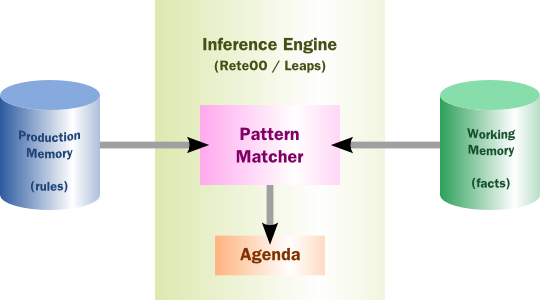
\includegraphics[width=12cm]{Pics/drools_abstract_structure.png}
			\caption{Architettura di Drools}
			\label{fig:DroolsArchitecture}
		\end{center}
	\end{figure}
	
	\begin{itemize}
		\item \textbf{Production Memory:} \\ Componente che contiene tutte le regole che compongono la Knowledge Base (KB);
		\item  \textbf{Working Memory: } \\ Componente che contiene tutti i fatti. In Drools, i fatti sono degli oggetti Java. \\  Si chiama \textit{Working Memory}, poiché  è possibile effettuare operazioni di modifica, inserimento e rimozione dei fatti che contiene;
		\item \textbf{Inference engine: } \\ Macrocomponente che ha la responsabilità di valutare i fatti della \textit{Working Memory} sulla base della Knowledge Base presente in \textit{Production Memory}. Per fare ciò si avvale di due sottocomponenti:
		\begin{itemize}
			\item \textbf{Pattern matcher: } \\ Componente che ha lo scopo di verificare, quando richiamata dall'inference engine, quali regole soddisfano la condizione presente nella \gls{LHS}\G\ sulla base dei fatti presenti nella  \textit{Working Memory} al momento dell'invocazione. Verranno poi eseguite le azioni  presenti nella \gls{RHS}\G\ di tali regole. Per fare ciò in modo efficiente con molti dati, viene utilizzato l'algoritmo Rete, brevemente descritto nell'\autoref{App:AppendiceAlgoritmoRete};
			\item \textbf{Agenda: } \\ Ha lo scopo di risolvere i conflitti tra le regole. Essi avvengono nel momento in cui più regole soddisfano la condizione nella loro \gls{LHS}\G\  con gli stessi fatti. \\ In questi casi, interviene l'Agenda che decide un ordine di esecuzione tra le regole che vanno in conflitto.
		\end{itemize}
	\end{itemize}
	
\paragraph{Vantaggi}
	\begin{itemize}
		\item In sistemi con grandi quantità di dati e vincoli, un approccio di questo tipo facilita notevolmente il mantenimento della verità ed il controllo sui dati inseriti. La definizione dei vincoli e l'aggiornamento degli stessi, risulta molto meno oneroso e di più facile verifica;
		\item L'elaborazione, risulta essere più veloce e performante rispetto ad un approccio tradizionale.
	\end{itemize}
\paragraph{Svantaggi}
	\begin{itemize}
		\item Per poter integrare questo sistema con Ruby on Rails é necessario utilizzare jRuby ed implementare in Java, le classi corrispondenti ai modelli sui quali si vogliono definire delle regole. Tecnicamente, qusto si fa con dei file di template java.erb di Rails che ottengono le informazioni riguardo classi e membri mediante \gls{reflection}\G;
		\item Per lavorare in modo efficace con questa tecnologia, è necessario investire molto tempo per conoscerne a fondo tutte le sfaccettature.
	\end{itemize}
\subsection{Foundation}
	\hl{Sezione nuovissima}
		\begin{figure}[H]
			\begin{center}
				
\includegraphics[width=7cm]{Pics/logo-foundation.png}
				\caption{Logo di Foundation}
				\label{fig:FoundationLogo}
			\end{center}
		\end{figure}
	Foundation è una collezione di \gls{framework}\G\ per lo sviluppo della componente \gls{front-end}\G\ di applicazioni web. \\ In particolare è composto da tre pacchetti:
	\begin{itemize}
		\item \textbf{Foundation for Sites: } per la realizzazione di siti web;
		\item \textbf{Foundation for Emails: } per la realizzazione di email formattate in html;
		\item \textbf{Foundation for Apps: } per la realizzazione di applicazioni web.
	\end{itemize}
	La struttura di ogni \gls{framework}\G\ è modulare e consiste essenzialmente di fogli di stile in formato \gls{SASS}\G\ - \gls{SCSS}\G. \\
	Per limitare il peso dei fogli di stile, è possibile selezionare  le sole componenti di cui si necessita al momento del download: saranno le sole presenti nel pacchetto da includere nel sito o da scaricare con un \gls{CDN}\G. \\
	Come la maggioranza dei \gls{framework}\G\ moderni per il \gls{front-end}\G\, Foundation fornisce un sistema di posizionamento a griglia dei componenti. Sono previste dodici colonne, visibili una accanto all'altra quando la larghezza dello schermo è maggiore di 940 pixel. Il numero di colonne viene adattato automaticamente a seconda dello spazio a disposizione, rendendo il sito, l'applicazione o l'email responsive. 
\paragraph{Vantaggi}
	\begin{itemize}
		\item Oltre ai comuni elementi HTML, sono messi a disposizione componenti aggiuntivi per la realizzazione delle sezioni di interfaccia maggiormente usate, ad esempio: 
		\begin{itemize}
			\item Gruppi di bottoni;
			\item Menu a tendina;
			\item \gls{Breadcrumb}\G;
			\item Messaggi formattati per avvisi, errori, aiuto.
		\end{itemize}\item Foundation permette di realizzare interfacce grafiche accattivanti senza dedicare eccessivo tempo alla loro implementazione;
		\item Questa collezione di \gls{framework}\G\ è stata testata sui principali \gls{browser}\G\ ottenendo ottimi risultati (vedi \autoref{fig:FoundationCompatibilita} per il dettaglio sulla versione utilizzata, la 5.5).
	\end{itemize}
	\begin{figure}[H]
		\begin{center}
			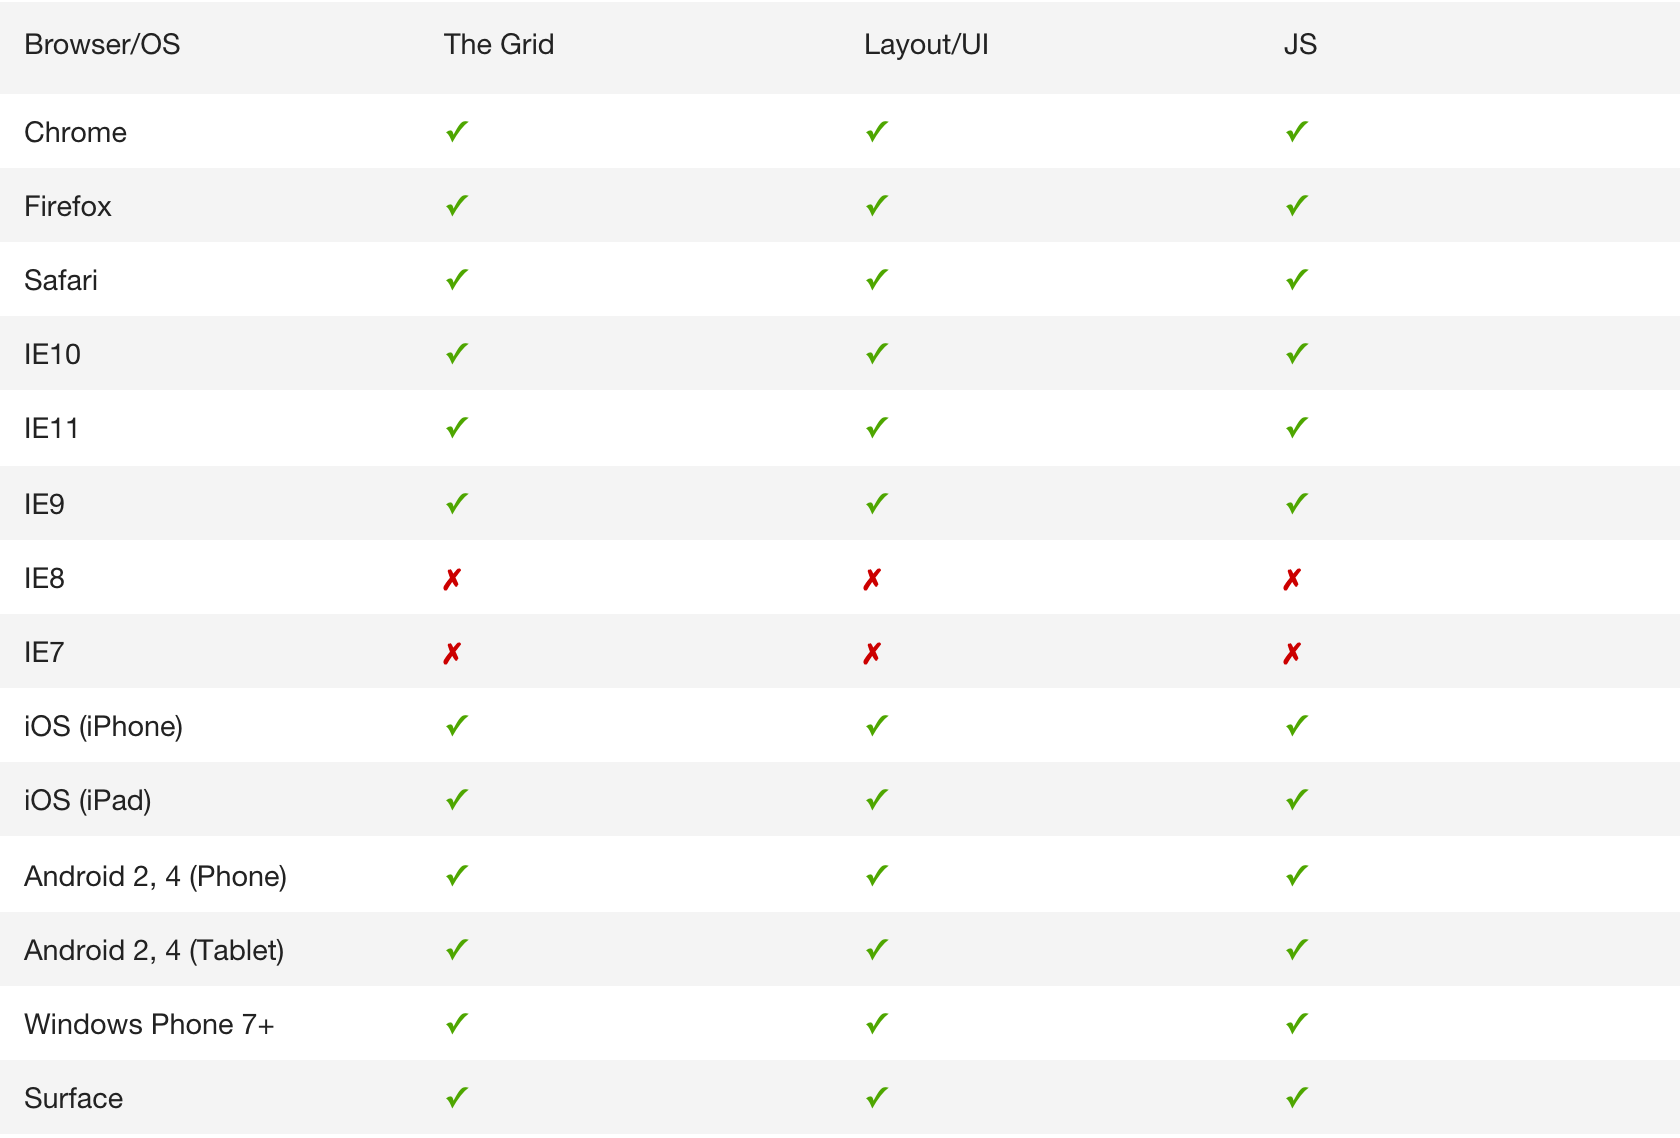
\includegraphics[width=15cm]{Pics/foundation5_compatibilita.png}
			\caption{Compatibilità di Foundation 5.5}
			\label{fig:FoundationCompatibilita}
		\end{center}
	\end{figure}
\paragraph{Svantaggi}
	\begin{itemize}
		\item Per utilizzare questo \gls{framework}\G\ è necessario investire del tempo per apprenderne appieno le caratteristiche.
	\end{itemize}
\subsection{jQuery}
	\hl{Sezione nuovissima}
	\begin{figure}[H]
		\begin{center}
			
\includegraphics[width=7cm]{Pics/jquery_logo.png}
			\caption{Logo di jQuery}
			\label{fig:jQueryLogo}
		\end{center}
	\end{figure}
	jQuery è una libreria \gls{javascript}\G\ per applicazioni web. Nasce con l'obiettivo di velocizzare l'attraversamento del \gls{DOM}\G  e semplificare la gestione delle chiamate \gls{Ajax}\G le degli eventi.
\paragraph{Vantaggi}
	\begin{itemize}
		\item Permette di eseguire chiamate \gls{Ajax}\G\ in modo veloce, rendendo così l'applicazione web più dinamica;
		\item Velocizza l'accesso e la gestione degli elementi del \gls{DOM}\G\ delle pagine \gls{HTML}\G;
		\item È stata testata sui principali \gls{browser}\G;
		\item Permette di semplificare e ridurre il codice, velocizzando il raggiungimento degli obiettivi. 
	\end{itemize}
\paragraph{Svantaggi}
	\begin{itemize}
		\item È sempre necessario importare tutto il pacchetto. Tuttavia, la versione compressa, occupa poco meno di 100 KiloBite. 
\end{itemize}
	\cleardoublepage
	
\section{Analisi del prodotto esistente}
\hl{sezione nuovissima}

Al momento dell'arrivo in azienda è già presente una versione alpha del software. \\
Sono attualmente supportate le aziende con i codici \gls{ATECO}\G\ in ambito edilizio, permettendo di gestire le informazioni relative a:
\begin{itemize}
	\item Sedi;
	\item Cantieri;
	\item Dipendenti;
	\item Organigramma aziendale;
	\item Abitabilità;
	\item Certificato di prevenzione degli incendi;
	\item \gls{DVR}\G\ e documentazione collaterale ad esso.
\end{itemize}
Il software espone una collezione di oltre 400 domande. Sulla base delle risposte a queste domande ed alle informazioni relative alle entità sopra indicate, vengono verificate alcuni vincoli mediante delle regole del sistema esperto.


\hl{[TODO ]}

\subsection{Architettura del software}
\subsubsection{Architettura ad alto livello}
\hl{sezione nuovissima}
Il software è gestito mediante tecnologia \gls{SaaS}\G, un modello di distribuzione del software applicativo dove il fornitore del software si occupa della sua implementazione e manutenzione. Il servizio viene erogato al cliente mediante una applicazione web fruibile via internet. \\ 
L'applicazione web risiede fisicamente su una macchina virtuale della piattaforma cloud \gls{AWS}\G, al fine di evitare oneri e spese di gestione di una infrastruttura informatica dedicata e garantire la scalabilità del servizio.\\

Come è possibile osservare da \autoref{fig:Architettura}, ogni istanza di macchina virtuale contiene un clone dell'intera architettura. È stata scelta questa soluzione perché è prevista la possibilità di vendere il pacchetto a più utenti che possono fungere da distributori.\\
Ogni istanza è composta da quattro componenti principali:
\begin{itemize}
	\item \textit{Rule Engine;}
	\item \textit{Database;}
	\item \textit{Web Application;}
	\item \textit{Storage.}
\end{itemize}
La componente \textit{Storage}, in particolare, è stata dedicata al salvataggio di documenti in formato PDF esportabili in ogni momento da ogni azienda. Questa funzionalità non è ancora stata implementata. \\
Il routing delle richieste viene effettuato con un \gls{reverse proxy}\G, nello specifico \textit{NGINX}. \\
In particolare Ruby on Rails permette nativamente di creare e versionare i database a seconda dell'ambiente nel quale si opera (\textit{development, test, staging e production}). Questa caratteristica è tornata molto utile per lo sviluppo, dal momento che è stato possibile fare test accurati senza intaccare i dati in produzione. Inoltre ciò rende possibile evitare di utilizzare la console in sandbox di Rails, la quale presenta criticità nella consistenza dei dati visibili da shell ripetto a quelli visibili da \gls{browser}\G. \\
La persistenza dei dati è stata gestita mediante il modulo \texttt{ActiveRecord} di Ruby on Rails (descritto nella sezione \ref{sec:ActiveRecord}) il quale salva le informazioni su un database \textit{ PostgreSQL}.
\begin{figure}[H]
	\begin{center}
		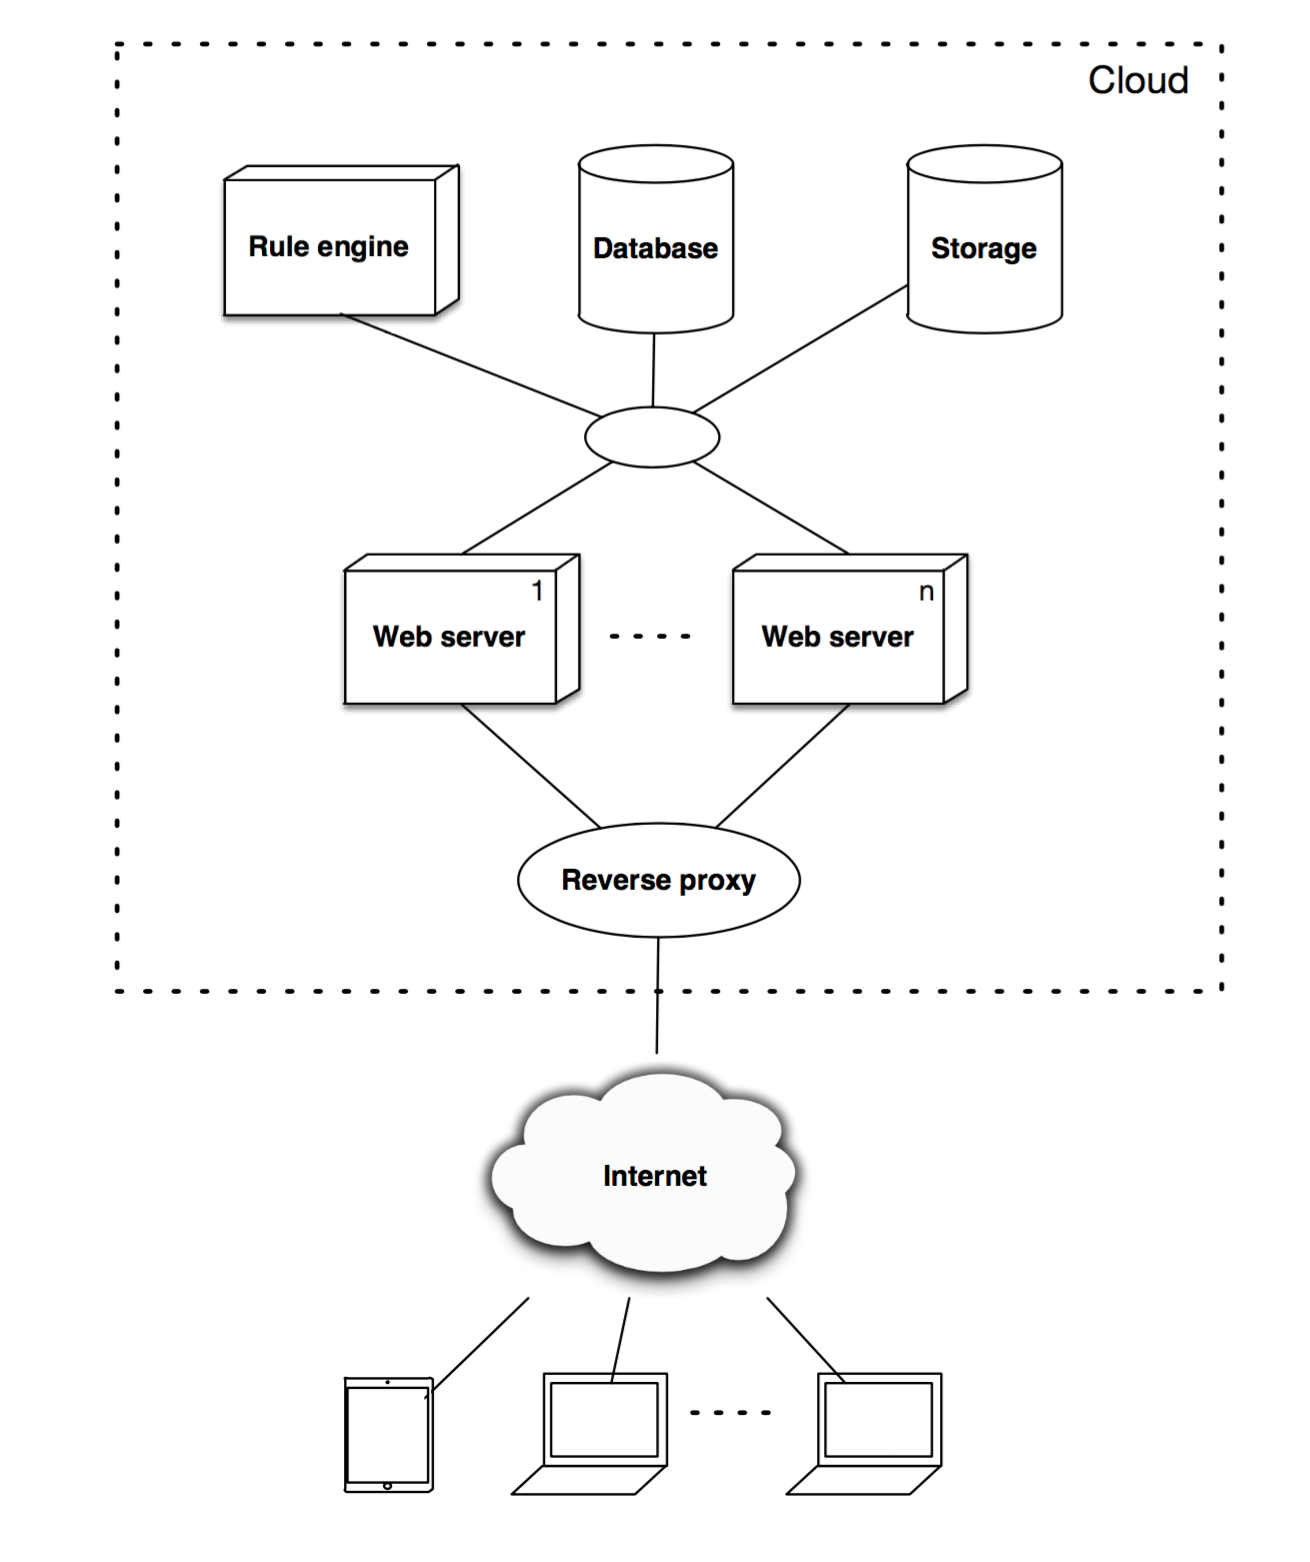
\includegraphics[width=12cm]{Pics/architettura.png}
		\caption{Architettura del sistema}
		\label{fig:Architettura}
	\end{center}
\end{figure}

\subsubsection{Architettura a basso livello}
\hl{sezione nuovissima}
L'applicazione web è organizzata secondo il pattern \gls{MVC}\G. Per il raggiungimento delle viste e l'accesso alle informazioni necessarie al corretto funzionamento dell'applicazione è stata implementata una interfaccia \gls{REST}\G. \\
Il sistema ha come entità principale il modello \texttt{Company} al quale sono riferite, direttamente o indirettamente, tutte le risorse.\\ 
Sono poi presenti numerosi modelli relativi alle entità che partecipano alla procedura di \gls{asseverazione}\G.
I modelli più significativi sono:
\begin{itemize} 
	\item \texttt{Alert} per rappresentare gli allarmi;
	\item \texttt{Answer} per rappresentare le risposte alle domande;
	\item \texttt{Company} per rappresentare una azienda;
	\item \texttt{ConstructionSite} per rappresentare un cantiere;
	\item \texttt{Dpi} per rappresentare un dispositivo di protezione individuale;
	\item \texttt{Duty} per rappresentare una mansione;
	\item \texttt{FireExtinguisher}  per rappresentare un estintore;
	\item \texttt{FirstAidBox} per rappresentare una cassetta di primo soccorso;
	\item \texttt{Individual} per rappresentare una persona;
	\item \texttt{Location} per rappresentare un edificio aziendale, ovvero una sede operativa, una sede amministrativa, una sede legale oppure un magazzino;
	\item \texttt{Machine, LiftingEquipment, ElectricTool}  per rappresentare un mezzo oppure uno strumento presente nel parco macchine;
	\item \texttt{MedicalVisit} per rappresentare una visita medica;
	\item \texttt{Procedure} per rappresentare una procedura aziendale, sia essa di prassi o di sistema;
	\item \texttt{Question} per rappresentare una domanda;
	\item \texttt{Training} per rappresentare un corso.
\end{itemize}	
Per ciascun modello, sono stati realizzati opportuni \textit{controller} e \textit{viste}. \\
Sono stati implementati, inoltre numerosi \gls{concern}\G\ per modularizzare le funzionalità indipendenti dalla singola classe ed allo stesso tempo riutilizzabili da altre classi. Ad esempio, ogni modello che, se istanziato, provoca un aumento del numero delle domande in attesa di risposta, include un apposito \gls{concern}\G\ per l'aggiornamento di un contatore dedicato a tale scopo. Per il calcolo del valore, il \gls{concern}\G\ ricava il nome della classe dell'oggetto corrente mediante \gls{reflection}\G\ ed incrementa automaticamente il valore del numero di domande correlate al tipo individuato.\\
\hl{[TODO finire di spiegare l'architettura ]}\\




\paragraph*{Relazioni tra domande, risposte ed allarmi}\mbox{} \\
\hl{sezione nuovissima}\\
Le risposte sono direttamente collegate alle domande ed ad una entità. Quando un utente risponde ad una domanda, viene aggiornato il recod relativo a quella risposta. A seguito di un inserimento o aggiornamento di una risposta, interviene Drools che valuta se le informazioni inserite rispettano tutti i vincoli previsti, altrimenti viene sollevato un allarme. \\ Per questioni di efficienza, gli allarmi relativi al vincolo di presenza  di una risposta, vengono gestiti direttamente dalle funzionalità di validazione di Rails.\\
Come per le answer, anche gli allarmi sono sempre collegati ad una risorsa, che di default è l'azienda corrente, ma può assumere come valore una qualsiasi istanza di un modello, purché non sia nulla.
Particolarmente degna di nota è l'associazione di una risposta o di un \textit{allarme} alla relativa risorsa. Per fare ciò si è utilizzato l'approccio standard di Rails per il supporto alle associazioni polimorfe. \\  Come si può vedere da  \autoref{fig:DiagrammaClassiAssociazioniPolimorfe}, indicando il tipo e l'id della risorsa interessata, l'accesso avviene tramite valutazione della classe e ricerca del relativo \textit{id}. \\
Si può pensare, ad esempio, all'allarme scatenato alla scadenza di un estintore. \\
La Risposta (\textit{Answer}) avrà i due campi \texttt{answerable\_type} ed \texttt{answerable\_id} impostati rispettivamente a \textit{"FireExtinguisher"} ed al suo \textit{id}.  L'allarme avrà un riferimento alla domanda per la quale è stata data una risposta. In questo modo è possibile conoscere il punto esatto dove dirottare l'utente al click sull'allarme per raggiungere il punto di non conformità. Questo aspetto è stato considerato di fondamentale importanza poiché la mole delle informazioni nel software è molto grande, è quindi necessario fornire il maggior numero di strumenti possibili all'utente per facilitarne la navigazione e l'orientamento nel sistema.
\begin{figure}[H]
	\begin{center}
		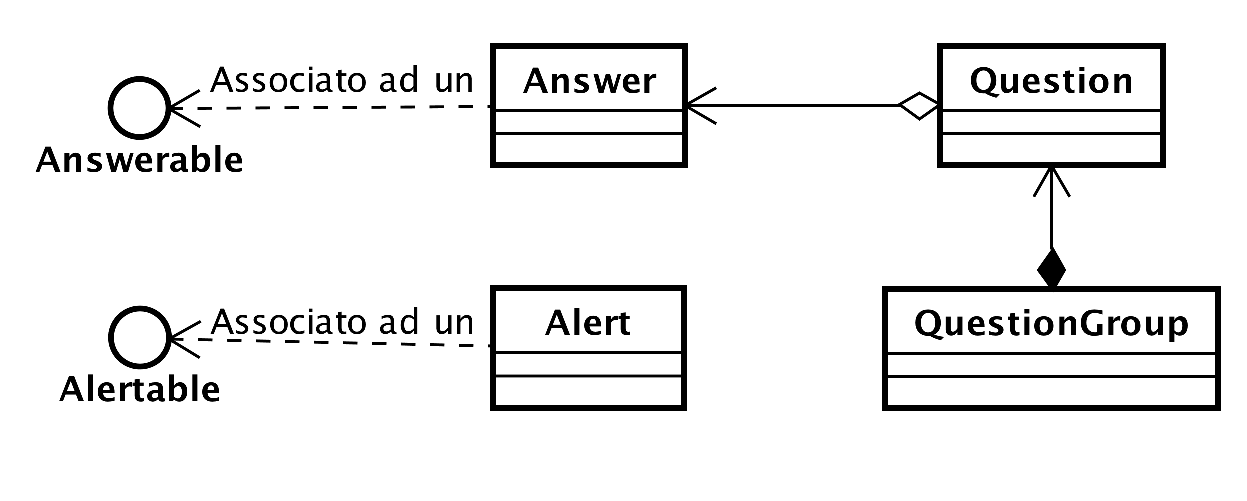
\includegraphics[width=14cm]{Pics/diagramma_classi_associazioni_polimorfe.png}
		\caption{Diagramma delle classi delle associazioni polimorfe di Risposte ed Allarmi.}
		\label{fig:DiagrammaClassiAssociazioniPolimorfe}
	\end{center}
\end{figure}

\subsubsection{Integrazione tra Ruby on Rails e Drools}\mbox{} \\
\hl{TODO scrivere meglio}
Il codice è stato scritto per la maggior parte utilizzando Ruby on Rails ma il rule engine (Drools) è un \gls{framework}\G\ scritto in Java. I due linguaggi non sono nativamente compatibili. \\
Per ovviare a questo problema, è stato utilizzato JRuby, un interprete del linguaggio Ruby scritto in Java, quindi in esecuzione su una \gls{JVM}\G\. \\
Per il corretto funzionamento di Drools, è necessario inserire le informazioni nella \textit{Working Memory} come \textit{"fatti"} che sono richiesti come oggetti di tipo \gls{JavaBean}\G\ o \gls{POJO}\G.\\
Per far cooperare i due ambienti, è stato implementato un apposito  \gls{concern}\G\ chiamato \texttt{"act\_as\_fact"}. Questo modulo viene incluso nelle classi delle quali è necessario tenere traccia nella \textit{Working Memory} e vengono generati, mediante reflection utilizzando i template di Rails (\gls{ERB}\G), le classi Java corrispondenti.




%\paragraph*{Criticità incontrate}\mbox{} \\
%\hl{SPOSTARE NELLA SEZIONE IN CUI SCRIVO QUELLO CHE HO FATTO IO}
%\hl{INSERIRE IL REMOTE TRUE NELLE VISTE}




\subsubsection{Flusso dei dati ed interazione}
\hl{Sezione nuovissima}
 Un aspetto che merita di essere esaminato è il flusso con il quale vengono generate e valutate domande e risposte  (\autoref{fig:DiagrammaAttivitaRisposte}).
\begin{figure}[H]
	\begin{center}
		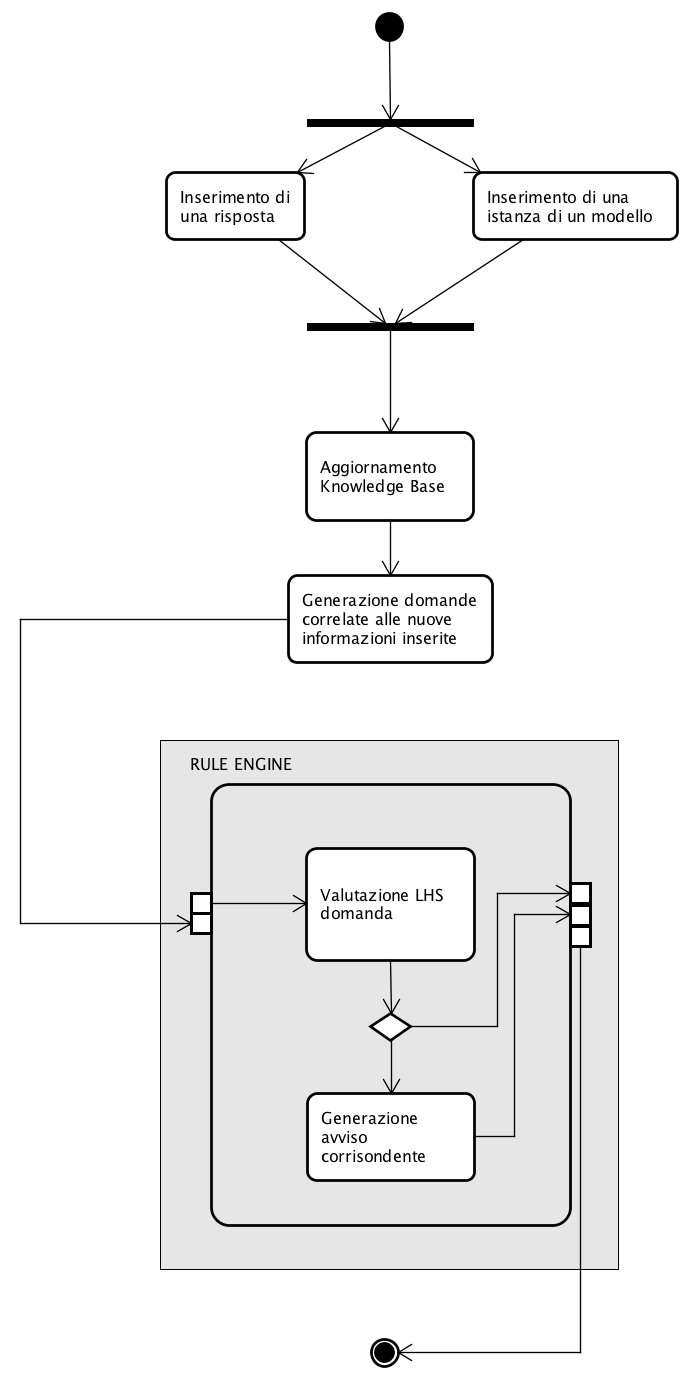
\includegraphics[width=8cm]{Pics/diagramma_attivita_risposte.png}
		\caption{Diagramma di attività del flusso di una risposta o l'inserimento di un oggetto a modello}
		\label{fig:DiagrammaAttivitaRisposte}
	\end{center}
\end{figure}

Nel momento in cui un utente inserisce o modifica un'istanza di un modello oppure risponde ad una domanda, viene aggiornata la \textit{Working Memory}. \\
Nel caso un cui venga generata o aggiornata un'istanza di modello, può essere necessario l'inserimento di alcune domande ad essa direttamente correlate.\\
Un esempio è rappresentato dall'aggiunta di un estintore ad un cantiere. Ad ogni estintore in ogni cantiere deve essere associata una posizione specifica che deve essere riportata nel layout di cantiere per permetterne il facile reperimento in caso di incendio. La posizione nel layout di un estintore è rappresentata dal software come una risposta ad una domanda in un apposito questionario generato ad ogni associazione di un estintore ad un cantiere. Se tale informazione non è specificata viene sollevato un allarme.\\
Sia per l'inserimento o aggiornamento di una risposta, sia per la generazione o modifica di una istanza di modello, il passo successivo è rappresentato dalla valutazione delle informazioni inserite sulla base della \textit{Knowledge Base}. \\
È in questo momento che agisce il rule engine Drools che per ogni regola presente nella \textit{Knowledge Base} valuta la \gls{LHS}\G\ sulle nuove informazioni inserite e, se soddisfatta, solleva gli allarmi corrispondenti. 
Un esempio di regola è il seguente:

\hl{TODO TABULAZIONI O LISTING CON AMBIENTE JAVA}
\begin{verbatim}
rule "Individuo ricopre una mansione per la quale non è formato"
	when
		$t: Training()
		$d: Duty(trainings contains $t)
		$i: Individual(duties contains $d, trainings not contains $t)
	then
		System.out.println($i.getFirstName() + ' ' + $i.getLastName() + "ha la mansione" +
		$d.getName() + " ma non la formazione " + $t.getName() );
end
\end{verbatim}
\begin{itemize}
	\item \$t contiene tutte le formazioni;
	\item \$d contiene  tutte le mansioni che necessitano della formazione \$t;
	\item \$i contiene tutti gli individui che svolgono la mansione \$d ma non sono in possesso della formazione \$t.
\end{itemize}
Le corrispondenze di questa regola sono tutti gli individui individui che svolgono una qualunque mansione per la quale non sono correttamente formati.\\
Al verificarsi di queste condizioni, viene generato un allarme il cui contenuto è specificato dalla stampa disposta dalla \gls{RHS}\G.



\section{Definizione dei casi d'uso}
	\subsection{Legenda}
	\subsection{UC 1}
	\subsection{UC 1.1}
	\subsection{UC 1.2}
	\subsection{UC 1.2.1}
	\subsection{UC 2}	
	\subsection{UC ...}

\section{Sviluppo}
\subsection{Refactor delle componenti esistenti}
	
\subsubsection{Refactor della componente: \textit{Figure di sistema}}
\subsubsection{Refactor della componente: \textit{Dispositivi di protezione individuale}}
\subsubsection{Refactor della componente: \textit{Mansioni e formazioni correlate}}
\subsection{Refactor della componente: \textit{Questionari}}


\subsection{Nuove componenti}
\subsubsection{\textit{Segnalazioni}}
	\paragraph{Requisiti}
	\paragraph{Progettazione}
	\paragraph{Criticità incontrate}
\subsubsection{\textit{Procedure}}
	\paragraph{Requisiti}
	\paragraph{Progettazione}
	\paragraph{Criticità incontrate}
		%più controller e viste associate allo stessa categoria, uno ha il modello l'altro il questionario
\subsubsection{\textit{Dispositivi di protezione collettivi}}
	\paragraph{Requisiti}
	\paragraph{Progettazione}
	\paragraph{Criticità incontrate}
		%remote true
		


\subsection{Regole Drools}
	
\section{Verifica e validazione}
\section{Considerazioni finali}
	\cleardoublepage
	%\input{tex/verifica.tex}
	\cleardoublepage
	%\input{tex/conclusioni.tex}
	\cleardoublepage

	\appendix
	\section{Migrazioni}

 \label{App:AppendiceMigrazioni}
Una migrazione è un file nel quale viene indicato cosa cambia nella struttura del database rispetto allo stato precedente ad essa e le variazioni ai dati ad essa conseguente.  Questo permette a tutti gli sviluppatori di avere lo stato della struttura del database sempre aggiornato.
Qui di seguito un esempio di migrazione che crea una tabella Bookmark (nel metodo statico up), e specifica cosa fare in caso di annullamento della migrazione (nel metodo statico down).
\begin{lstlisting}
class CreateBookmarks < ActiveRecord::Migration
  def self.up
    create_table :bookmarks do |t|
      t.string :url
      t.string :title
      t.text :description
      
      t.timestamps
    end
  end

  def self.down
    drop_table :bookmarks
  end
end
\end{lstlisting}
Una volta eseguita la migrazione verrà creata una tabella Bookmarks con i tre campi \textit{url}, \textit{title} e \textit{description}.
	\cleardoublepage
	\section{Inferenza e Motori di inferenza}

 \label{App:AppendiceInference}
 Con  il termine inferenza si intende il processo con il quale si passa da una proposizione vera ad una seconda proposizione la cui verità è derivata dal contenuto della prima. \\
 Questo processo avviene mediante l'applicazione di regole, dette regole di inferenza. Al verificarsi di una o più condizioni (\textit{antecedent}), queste regole traggono delle conclusioni ed agiscono di conseguenza sul sistema, sulla base di ciò che è definito nella seconda parte della regola (\textit{consequent}).\\
 \hl{Prendiamo ad esempio la regola \texttt{"Se piove apro l'ombrello"}. \\ L'\textit{antecedent} è rappresentato dalla condizione: \texttt{"Oggi piove?"}. Se la condizione dell'\textit{antecedent} è soddisfatta, verrà tratta la conclusione descritta nel \textit{consequent}, in questo caso \texttt{"apro l'ombrello"}. }
 
 Questo genere di approccio assume maggior significato se applicato contemporaneamente ad un insieme di fatti o circostanze. \\
 Un motore inferenziale (\textit{inference engine}), è un software il cui algoritmo simula le modalità con cui la mente umana trae delle conclusioni logiche attraverso il ragionamento utilizzando le regole di inferenza.
 Le due modalità con cui si opera in questi contesti sono principalmente le seguenti:

\begin{itemize}
	 
	 \item \textbf{Backward chaining} \\
	 Rappresenta il ragionamento di tipo induttivo, il quale dall'analisi di informazioni di carattere particolare permette di ricavare informazioni di carattere generale. \\
	 Nella pratica, si considerano una serie di obiettivi e si cerca tra i dati disponibili se ce ne sono di disponibili tali da supportare tutti gli obiettivi fissati.\\
	 Un motore inferenziale utilizza questo approccio cercando tra le regole di inferenza finché non ne individua una che abbia il \textit{consequent} che soddisfa l'obiettivo.
	 Se non è provata la verità dell'\textit{antecedent} della regola individuata, allora l'\textit{antecedent} stesso diventa un nuovo obiettivo poiché, una volta soddisfatto, sarà soddisfatto anche l'obiettivo precedentemente individuato.  
	 
	 
	\item \textbf{Forward chaining} \\
	 Rappresenta il ragionamento di tipo deduttivo, ovvero permette di partire da principi di carattere generale per estrarne uno o più di carattere particolare.\\
	 L'approccio utilizzato è quello di iniziare con i dati già disponibili ed usare le regole di inferenza per estrarne di nuovi fino a quando non si è raggiunto l'obiettivo fissato.\\
	 Un inference engine che usa il forward chaining, itera sulle regole di inferenza eseguendo quelle che hanno disposizione tutte le informazioni per poter calcolare i nuovi dati  e fermandosi quando è stato raggiunto l'obiettivo fissato.  \\
	 A differenza del backward chaining, questo è un approccio orientato ai dati ed effettua i \textit{"ragionamenti"} al fine di ottenere delle risposte. \\
	 È consigliabile rispetto al backward chaining nelle situazioni in cui i dati cambiano frequentemente, perché in seguito alla modifica, alla cancellazione ed all'immissione di nuovi dati, viene innescato il processo di inferenza dilazionando il costo computazionale nel tempo.
\end{itemize} 
 
 
 

	\cleardoublepage
	\section{Sistemi Esperti}
\hl{NUOVA SEZIONE}
 \label{App:AppendiceSistemiEsperti}
 
 Un sistema esperto è un programma che cerca di riprodurre le prestazioni di una o più persone esperte in un determinato campo di attività. \\
 Per il corretto funzionamento, è necessario che siano fornite procedure di inferenza sufficienti alla risoluzione dei problemi alla quale si vuole fornire risposta. \\
 Un sistema esperto, è sempre in grado di esibire i passaggi logici che hanno portato ad una particolare decisione.
 Le principali componenti sono: 
 \begin{itemize}
 	\item \textbf{Base di conoscenza(Knowledge Base):}\\
	 	Componente che contiene tutto ciò che serve al sistema per prendere le decisioni (e non i dati); 
	\item \textbf{Motore inferenziale}\\
	  (vedi \autoref{App:AppendiceInference});
	\item \textbf{Interfaccia Utente}
		Componente che permette l'interazione fra il soggetto umano ed il software che deve dare risposta ad un suo particolare problema.
 \end{itemize}
 
 
 I sistemi esperti si dividono in due categorie principali: basati su regole oppure su alberi. 
 Per la realizzazione del progetto di stage è stato utilizzato \textit{Drools}, che si basa su regole. Non verranno quindi trattati su questa tesi i sistemi basati su alberi.\\
 I sistemi esperti basati su regole sono dei programmi composti da regole della forma \texttt{IF condizioni THEN azione}. La parte condizionale viene detta Left Hand Side (LHS), mentre quella relativa all'azione viene detta Right Hand Side (RHS).\\
 Le regole vengono verificate ogni volta che i dati subiscono un cambiamento. Questo avviene mediante l'introduzione di nuovi fatti.\\
 Esempio:
	 Fatti 
	 \begin{itemize}
	 	\item Mal di Testa
	 	\item Raffreddore
	 	\item Temperatura >=38
	 \end{itemize}
 \begin{lstlisting}
	IF( (Mal di testa) AND (Raffreddore) AND (Temperatura >=38))
	THEN ( Diagnosi: Influenza)
 \end{lstlisting}

 
 

%portare nella sezione tecnologie


\section{Fnzionamento di Drools} 


 \subsection{Algoritmo RETE}
 L'algoritmo RETE è stati inventato da Charles Forgy nel 1978-79.. \\
 Può essere separato in due parti:
 \begin{itemize}
 	\item Compilazione delle regole;
 	\item Esecuzione runtime.
 \end{itemize}
 Questo algoritmo prevede l'utilizzo di una sorta di rete che filtra i dati mano a mano che essi la attraversano. I nodi all'inizio della rete avranno, con probabilità molto alta, un numero elevato di match. 
 Mano a mano che si scende in profondità, le corrispondenze tenderanno sempre più a diminuire di numero. In fondo alla rete, troveremo i nodi terminali. \\
Il funzionamento prevede la creazione di un nodo radice, attraverso il quale tutti gli oggetti entrano nella rete. Ogni oggetto, dopo essere passato per il nodo radice, viene subito indirizzato verso un altro nodo chiamato \textit{ObjectTypeNode} che ha lo scopo di assicurare che ogni nodo venga inoltrato verso nodi che sanno gestire oggetti con un tipo compatibile a quello dell'oggetto in analisi\footnote{Tecnicamente questo passaggio avviene mediante l0'invocazione dell'operatore \texttt{instanceof} di Java.}.\\
Gli ObjectTypeNode, possono propagare gli oggetti verso tre tipologie di nodi:
\begin{itemize}
	\item AlphaNodes
	\item LeftIUnputAdapterNodes
	\item BetaNodes
\end{itemize}
 
 \subsection{Production Memory}
 
 \subsection{Working Memory}
 
 \subsection{Agenda}
 
 \subsection{Hybrid Reasoning}
 Drools usa prima uno poi l'altro \textcite{eco:tesi} \\
 TODO
	\cleardoublepage
	\section{Algoritmo RETE}
 \label{App:AppendiceAlgoritmoRete}
 	L'algoritmo RETE è stato inventato da Charles Forgy nel 1978 e successivamente perfezionato nel 1979. \\
 	Può essere separato in due parti:
 	\begin{itemize}
 		\item Compilazione delle regole;
 		\item Esecuzione runtime.
 	\end{itemize}
 	Questo algoritmo prevede l'utilizzo di una sorta di rete che filtra i dati mano a mano che essi la attraversano. I nodi all'inizio della rete avranno, con probabilità molto alta, un numero elevato di match. 
 	Mano a mano che si scende in profondità, le corrispondenze tenderanno sempre più a diminuire di numero. In fondo alla rete, troveremo i nodi terminali. \\
 	Il funzionamento prevede la creazione di un nodo radice, attraverso il quale tutti gli oggetti entrano nella rete. Ogni oggetto, dopo essere passato per il nodo radice, viene subito indirizzato verso un altro nodo chiamato \textit{ObjectTypeNode} che ha lo scopo di assicurare che ogni nodo venga inoltrato verso nodi che sanno gestire oggetti con un tipo compatibile a quello dell'oggetto in analisi\footnote{Tecnicamente questo passaggio avviene mediante l'invocazione dell'operatore \texttt{instanceof} di Java.}.\\
 	Gli \textit{ObjectTypeNode},  propagano gli oggetti verso dei nodi detti \textit{AlphaNode}, ognuno dei quali verifica una condizione. \\
 	Tramite altre due tipologie di nodi (\textit{JoinNode} e \textit{NotNode}), si verificano condizioni che coinvolgono oggetti di diverso tipo, per poi giungere infine ai nodi terminali. \\
 	Una volta raggiunto un nodo terminale, si ha la garanzia che la regola è stata soddisfatta e viene eseguita l'azione descritta nella \gls{RHS}\G\ corrispondente.
 	%valutare se andare in profondità o meno
 	
 	
 	\begin{figure}[H]
 		\begin{center}
 			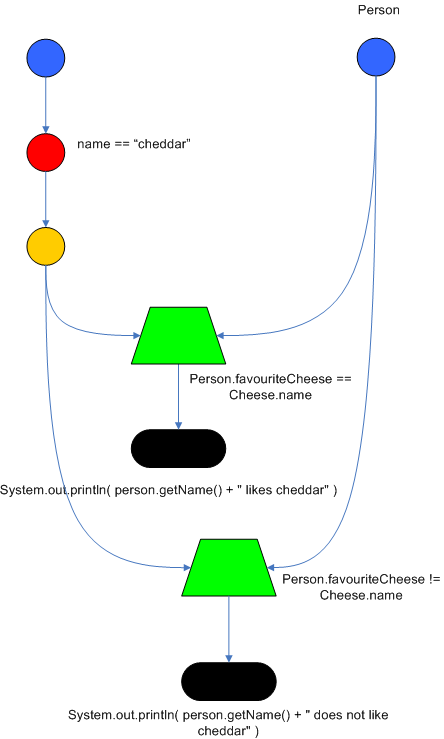
\includegraphics[width=12cm,height=12cm,keepaspectratio]{Pics/drools_rule_flow_example.png}
 			\caption{Esempio di flusso di valutazione di una regola Drools.}
 			\label{fig:DroolsRuleEvalFlow}
 		\end{center}
 	\end{figure}
 	
 	Un esempio di flusso di funzionamento è raffigurato nella \autoref{fig:DroolsRuleEvalFlow}. \\
 	In particolare i nodi azzurri sono degli \textit{ObjectTypeNode} e rappresentano nell'ordine formaggi e persone. \\
 	Il nodo rosso, invece, è di tipo \textit{AlphaNode} e verifica la condizione che il nome del formaggio sia "cheddar". \\
 	Il nodo giallo è di tipo \textit{LeftInputAdapterNode} e serve per scegliere dove dirottare il flusso a seguito del soddisfacimento o meno di una condizione prevista da un \textit{AlphaNode}.\\
 	Se la condizione prevista dall'\textit{AlphaNode} è verificata, il flusso viene inoltrato al primo punto di join (identificato da un trapezio verde) che verifica se il formaggio preferito dalla persona è il \textit{cheddar}. si dice punto di join perché per operare ha bisogno delle informazioni provenienti da due diverse entità gestite da degli \textit{ObjectTypeNode} distinti. \\ se la condizione prevista dall'\textit{AlphaNode} non è verificata, si passa al secondo punto di join.\\
 	In caso di verifica delle condizioni dei \textit{JoinNode}, si giunge ai nodi terminali ovvero al soddisfacimento delle condizioni che permette di prendere una decisione. In questo caso viene solo stampata una stringa, ma in generale è possibile scegliere l'azione più adatta al contesto di utilizzo.

 	
 	
 	
 	
 	
 	
 	
 	
 	
 	
 	
 	
 	
 	
 	
 	
 	
 	
 	
 	
 	
 	
 	
 	
 	
 	
 	
 	
 	
 	
 	
 	
 	
	
	
	
	%\input{tex/database.tex}
	\clearpage
	%\input{tex/backend.tex}
	\cleardoublepage

	\printglossaries
	\addcontentsline{toc}{section}{\refname}

%	\bibliography{bibliografia}
%	\bibliographystyle{plainnat}
\end{document}
